\chapter{Literature Review}
\label{chap: 2}

\section{Scope and Goal for literature review}
\label{sect: 2.1scope}

This chapter provides an overview of the current knowledge and available literature on accelerated CFD simulations. As a start, \autoref{sect: 2.2turbflows} explains the most used ways in which turbulent simulations can be resolved. Next \autoref{sect: 2.4performance enhancing} and \autoref{sect: 2.5ML enhancing} will explain the various ways CFD simulations have been enhanced. Where \autoref{sect: 2.4performance enhancing} will introduce conventional ways of enhancing simulations, and \autoref{sect: 2.5ML enhancing} will introduce how current advances in machine learning and artificial intelligence are being incorporated in the current CFD landscape.  

% \subsection{Methodology}
% The literature review presented in this chapter was conducted with the aim of crafting a strong understanding of current advances in the field of accelerating CFD simulations. The primary tools used for sourcing the material discussed in this review were \textit{Google scholar}, \textit{Litmaps}, \textit{TuDelft Library} and conventional google search queries. The selected material was evaluated based on relevance to the thesis subject, amount of citations, the reputation of the journal it was published in, expertise of authors and date of publication. This way the most relevant material in the field could be referenced in this literature review. 

\section{Turbulent flows: simulation and modelling}
% This section aims to provide an overview on the mathematical frameworks behind CFD and how turbulent flows can be represented and modelled. Beginning with the governing equations for turbulent flows and moving on to how these equations have been adapted to a solvable models. This section aims to provide a preliminary outlook of the most used types of CFD frameworks that have been implemented over time.

\label{sect: 2.2turbflows}
Fluid dynamics is governed by a set of coupled partial differential equations (PDE's) called the Navier-Stokes Equations (NSE). These equations are based on the assumptions of conservation off mass and momentum. These equations are shown in \ref{eq: navier-stokes} in \textit{Einstein notation} \cite{Turbulence}. Note that the equations seen in \ref{eq: navier-stokes} display the governing equations of a fluid of which we have assumed a constant density, which means that density $\rho$ is a material property and not something that needs to be solved for.

\begin{subequations} \label{eq: navier-stokes}

    % Continuity
    \begin{equation} \label{eq: continuity}
    \begin{aligned}
    \frac{\partial u_i}{\partial x_i} &= 0
    \end{aligned}
    \end{equation}

    % Momentum
    \begin{equation} \label{eq: momentum}
    \begin{aligned}
   \underbrace{ \frac{\partial u_i}{\partial t} }_{\text{Local acceleration}}
+ 
\underbrace{ u_j \frac{\partial u_i}{\partial x_j} }_{\text{Convective term}}
= 
\underbrace{ -\frac{1}{\rho} \frac{\partial p}{\partial x_i} }_{\text{Pressure gradient}}
+ 
\underbrace{ \nu \frac{\partial^2 u_i}{\partial x_j \partial x_j} }_{\text{Viscous diffusion}}
+ 
\underbrace{ g_i }_{\text{Body forces}}
    \end{aligned}
    \end{equation}
\end{subequations}

Where $u$ is the 3-dimensional velocity vector, $x$ is the position vector, $p$ is the pressure in the fluid, $\nu$ is the kinematic viscosity of the fluid, $g$ is the gravitational constant, $t$ is time and finally the subscripts $i$ and $j$ indicate spatial directions.

These equations have proven to be a tough fluid dynamics challenge and have yet to be solved analytically. Due to their non-linearity and strong coupling, they display complex behaviour. This behaviour mainly arises from the non-linear convective term in the momentum equation. This fact is particularly pronounced for high Reynolds number flows, where small-scale turbulent structures dominate \cite{Turbulence}. In the current field of mathematics, solutions to the most fundamental questions regarding the NSE remain unanswered. Questions such as: do solutions exist, and are they unique \cite{clay_navierstokes}? It is due to this complexity and lack of understanding that the Clay Mathematics Institute has listed the NSE as one of the 7 Millennium Problems. Because of the absence of an analytical solution, engineers and researchers must discretise, model, and make assumptions about various parts of the NSE to find a numerical solution to these equations. 

\subsection{DNS}
One way to evaluate the NSE is through a Direct Numerical Simulation (DNS). A DNS aims to capture all length and timescales of a turbulent flow directly, without modelling and without further assumptions. Furthermore, DNS must accurately resolve the temporal resolution of the turbulent flow it aims to simulate. Following Kolmogorov's microscale hypothesis \cite{Kolmogorov1941} and the two-point correlation function \cite{Pope2000}, the smallest and largest turbulent length scales can be obtained, respectively. Using these length scales, the mesh spacing and mesh dimensions can be determined; this way, all relevant length scales can be represented in the turbulent flow field without resorting to modelling. These length scales are strongly correlated to the Reynolds numbers, which is the ratio of inertial forces and viscous forces. 

\begin{equation}\label{eq: Reynoldsnr}
    Re = \frac{\text{Inertial forces}}{\text{Viscous forces}}= \frac{u l}{\nu}
\end{equation}

Where $u$ is the flow velocity and $l$ is the characteristic length. At large Reynolds numbers, turbulent flows exhibit a wide range of scales, where the smallest turbulent length scales become progressively smaller as $Re$ increases. This means that for a high $Re$ DNS, a very fine mesh would need to be generated. 

In fact, when following Kolmogorov in assuming the smallest scales of turbulence are universal and isotropic, the total number of grid points (degrees of freedom) required for a DSN scales with $Re^{9/4}$ \cite{Coleman2010}. Factoring in the necessary change in timestep to maintain a constant CFL number, the total computational effort for DNS would be equal to $\mathcal{O}(Re^3)$ \cite{Coleman2010}. This extensive computational requirement makes DNS highly accurate but prohibitively expensive for general practical use. However, it remains indispensable for fundamental turbulence research due to its ability to provide complete knowledge of the flow without empirical approximations.


\subsection{RANS}
One way to reduce the computational cost of numerical simulations of the NSE was stipulated by \textcite{Reynolds1895} in 1895. In this work, he proposed decomposing the instantaneous velocity into two distinct parts: the time-averaged part and the fluctuating part. 

\begin{equation}\label{eq: ReDecompose}
    u_i = \langle u_i \rangle + u_i'
\end{equation}

\begin{wrapfigure}{r}{0.45\textwidth}
\vspace{-2em}
    \centering
    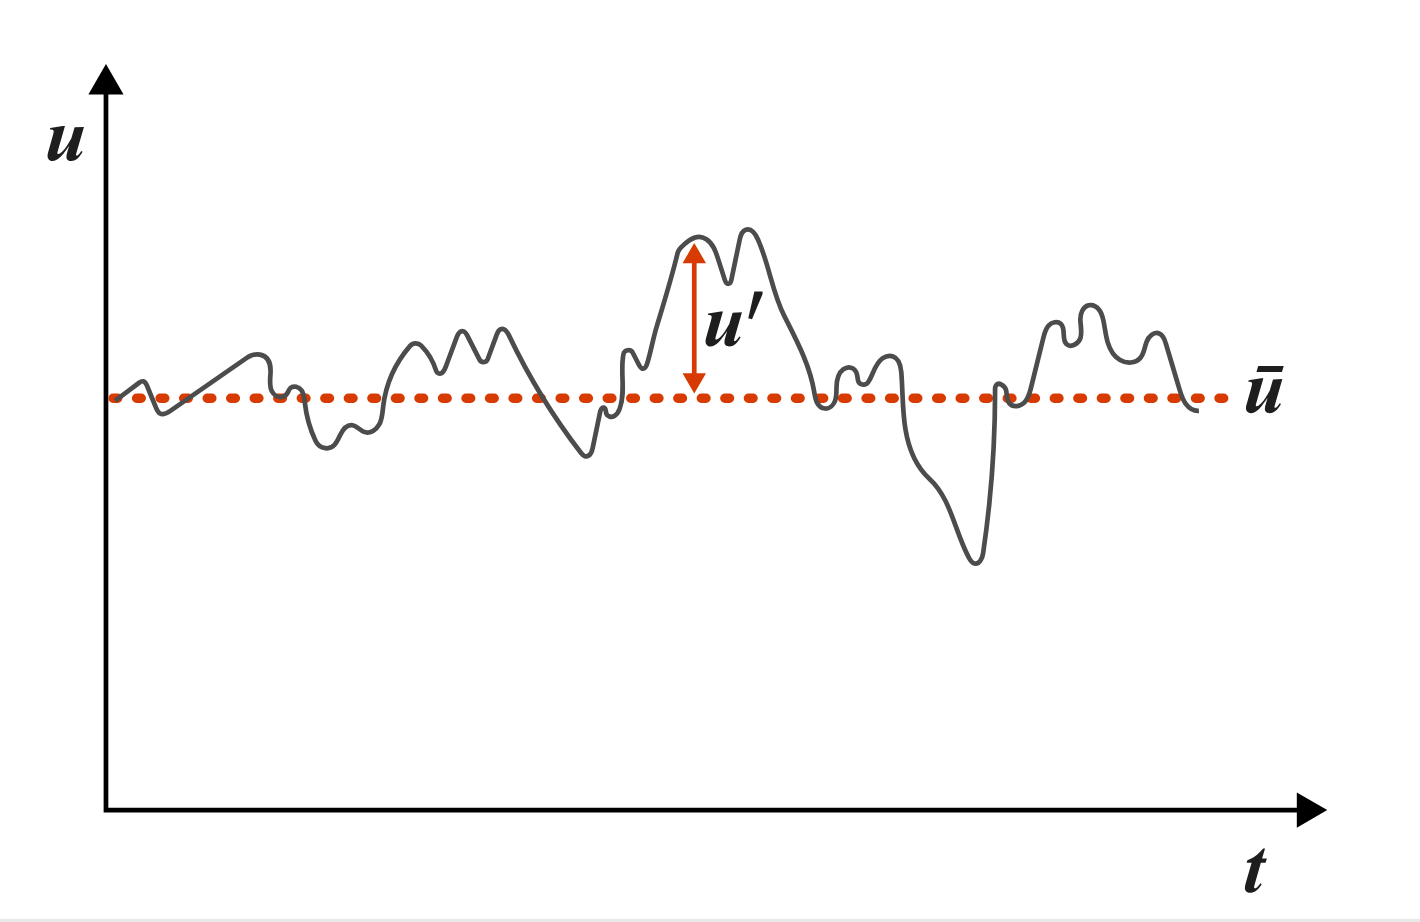
\includegraphics[width=\linewidth]{figures/Literature review/RANS.png}
    \caption{Schematic of the Reynolds decomposition for incompressible flow: the instantaneous velocity $u(t)$ (solid line) is split into its time‐averaged mean $\overline{u}$ (dashed red line) and the fluctuation $u'(t)=u(t)-\overline{u}$. Adapted from \cite{Altair2021RANS}}    
  \label{fig: rans}
  \vspace{-2em}

\end{wrapfigure}

In \autoref{eq: ReDecompose}, the instantaneous velocity $u_i$ is decomposed into the time-averaged part $\langle u_i \rangle$ and the fluctuating component $u_i'$.1 This decomposing into time-averaged and fluctuating parts is called \textit{'Reynolds decomposition'}. Substituting \autoref{eq: ReDecompose} into \autoref{eq: navier-stokes} results in the incompressible Reynolds Averaged Navier Stokes (RANS) equations \cite{FiniteVolume}. Because the time averaging in the Reynolds decomposition is much larger than the largest timescale of the turbulent fluctuations, the evolution of the mean flow component can be determined \cite{Roelofs2019}. However, this also means that none of the turbulent fluctuations are resolved; instead, turbulent scales are modelled through a closure model, which must provide a suitable representation of the effects of these fluctuations on the mean flow.


% \pagebreak

After applying the substitution, \autoref{eq: RANS} can then be solved to obtain the time-averaged solution of the NSE.

\pagebreak
\begin{subequations} \label{eq: RANS}

    % Continuity
    \begin{equation} \label{eq: RANSCont}
    \begin{aligned}
    \frac{\partial \langle u_i \rangle}{\partial x_i} &= 0
    \end{aligned}
    \end{equation}

    % Momentum
    \begin{equation} \label{eq: RANSMomentum}
    \begin{aligned}
   \frac{\partial \langle u_i \rangle}{\partial t} 
   + 
   \langle u_j \rangle \frac{\partial \langle u_i \rangle}{\partial x_j} 
   &= 
   -\frac{1}{\rho} \frac{\partial \langle p \rangle}{\partial x_i} 
   + 
   \nu \frac{\partial^2 \langle u_i \rangle}{\partial x_j \partial x_j}
   + 
   g_i
    -
   \frac{\partial \langle u_i' u_j' \rangle}{\partial x_j}
    \end{aligned}
    \end{equation}
\end{subequations}

These incompressible RANS equations are similar to the conventional NSE seen in \autoref{eq: navier-stokes}, the only difference being the addition of the divergence of the averaged products of the Reynolds stress tensor: $\frac{\partial \langle u_i' u_j' \rangle}{\partial x_j}$. To ensure accurate results, the effect of the Reynolds Stress Tensor (RST) needs to be modelled by turbulence models. Because the time-dependent fluctuations are not being resolved, RANS simulations can be executed on grids with a larger mesh spacing, which inherently reduces the amount of required operations and thus the computational cost. 

To achieve accurate simulations, the effect of the RST needs to be modelled. The most used models are those of \textcite{Launder1974}, \textcite{Wilcox1988}, \textcite{Spalart1992e}, \textcite{Launder1975} and \textcite{Speziale1991}. 


\subsection{LES}
Another widely implemented turbulent flow framework was initially proposed by \textcite{Smagorinsky1963} to stabilise under-resolved weather simulations. This proposition was later applied to engineering-related flows by \cite{Deardoff1970} and subsequently by \textcite{Schumann1975}. In this work, the proposition was made only to resolve the large-scale turbulent structures of the flow, while modelling the effect of the small-scale structures. Because only the large-scale eddies are being resolved in this simulation, this type of simulation is called a Large Eddy Simulation (LES). The governing equations of LES are determined by applying a low-pass filter operation to \autoref{eq: navier-stokes}, which results in the governing equations seen in \autoref{eq: LES}. After the filtering operation has been applied, a sort of 'smooth' version of the velocity fluctuations is achieved, which is displayed in figure \autoref{fig: LES}. 


\begin{subequations} \label{eq: LES}
    % Continuity
    \begin{equation} \label{eq: LESCont}
    \begin{aligned}
    \frac{\partial  \overline{u}_i }{\partial x_i} &= 0
    \end{aligned}
    \end{equation}

    % Momentum
    \begin{equation} \label{eq: LESMomentum}
    \begin{aligned}
   \frac{\partial \overline{u}_i}{\partial t} + \overline{u}_j \frac{\partial \overline{u}_i}{\partial x_j} = 
-\frac{1}{\rho} \frac{\partial \overline{p}}{\partial x_i} 
+ \nu \frac{\partial^2 \overline{u}_i}{\partial x_j \partial x_j} 
+ g_i 
- \frac{\partial \tau_{ij}}{\partial x_j}
    \end{aligned}
    \end{equation}
\end{subequations}

\begin{wrapfigure}{r}{0.45\textwidth}
\vspace{-1em}
    \centering
    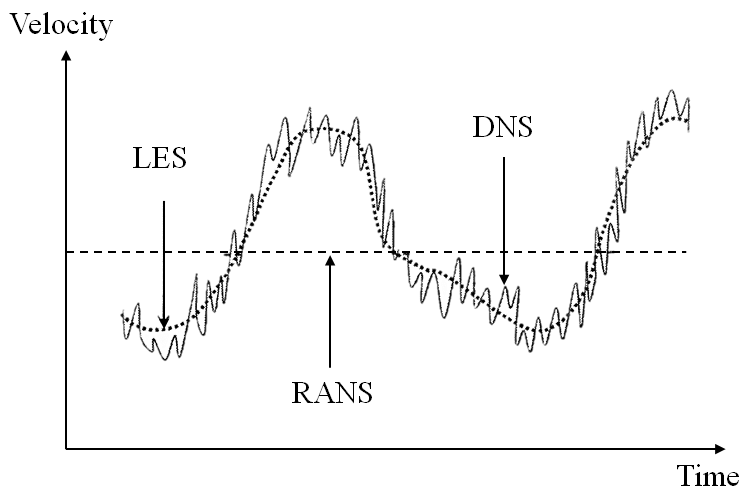
\includegraphics[width=\linewidth]{figures/Literature review/LES.png}
    \caption{Comparison of turbulence modelling approaches based on their resolution of velocity fluctuations over time. DNS captures all spatial and temporal fluctuations, while LES resolves only the large-scale fluctuations. Adapted from \cite{Foale2021}}    
  \label{fig: LES}
\vspace{-1em}
\end{wrapfigure}

Where $\overline{u}_i$ is the filtered velocity. The filter operation is applied through a filter kernel $G$, where the filter cut-off width is determined to be proportional to the grid size. As seen in \autoref{eq: LESMomentum}, a new term arises $\frac{\partial \tau_{ij}}{\partial x_j}$, which contains the effects of the turbulent scales that the filter operation has cut off. Because most energy is dissipated from a flow in the most minor scales \cite{Turbulence}, this 'Sub Grid Scale' (SGS) tensor needs to be modelled in such a way that it artificially drains enough energy from resolved scales. Many different kinds of SGS models have been proposed, most of which utilise an 'Eddy viscosity' to equate the amount of energy drained to the strain the fluid experiences. The most used eddy viscosity models are ones like the Smagorinsky model (\textcite{Smagorinsky1963}), the  Scale Similarity Model (\textcite{Bardina1980}), the Dynamic Smagorinsky Model (\textcite{Germano1991}, \textcite{Lilly1992}), the Wall-Adapting Local Eddy-viscosity model (\textcite{Nicoud1999}) and the Vreman model (\textcite{Vreman2003}).

Because the large-scale structures are directly resolved, LES is more accurate than the RANS approach when applied to the same flow case, as these large structures contain most of the turbulent kinetic energy and are responsible for the majority of momentum transfer and mixing. Because the accuracy of LES is determined by the filter width, which is in turn related to the grid spacing, grid refinement will lead to more accurate LES results. At the same time, refinement will also significantly increase the computational cost of the simulation. That is why for high-accuracy flow cases, acceleration frameworks are of high necessity to keep computation cost within usable limits. 

Since the concept of LES was proposed in 1963, it has undergone significant evolution and gained wider acceptance, particularly in academic and research settings. Despite the increase in computational power over the past few decades \cite{Shalf2020}, the cost of performing LES remains higher than that of comparable simulations using the RANS framework. This higher cost is due to the need for LES to explicitly resolve the temporal evolution of larger turbulent eddies, which requires finer grid resolutions and more time steps, in contrast to RANS, where the equations are time-averaged and all turbulent fluctuations are modelled.

However, recent academic advancements in LES frameworks, such as those highlighted by \textcite{Weymouth2025}, suggest that LES can be conducted at a relatively low computational cost, even with limited knowledge of the methodology. This perspective aligns with the assertion made by \textcite{Piomelli2014}, who stated that “LES will be used in more complex configurations and will yield reliable results for engineering analysis.”

Despite the high computational cost of LES, advancements in modelling and algorithm design will continue to reduce the cost of high-fidelity simulations. That is why, contrary to \textcite{Zhiyin2015}, we expect that LES will be more widely adopted in general engineering instances. Even more so with the acceleration frameworks discussed in further section, \ref{sect: 2.4performance enhancing} and \ref{sect: 2.5ML enhancing}.

\section{Performance enhancing in CFD}
\label{sect: 2.4performance enhancing}

Even with the significant computational cost improvements that RANS offers and the advances in LES frameworks, there remains a need for further computational enhancements in high-fidelity applications. While RANS models reduce computational costs by utilising turbulence models, they often compromise accuracy. LES significantly improves accuracy, but remains expensive for high Reynolds number flows. This is especially the case for wall-bounded flow cases, where the computational time scales using $Re^{2.4}$ for wall-resolved meshes. In an attempt to bridge the trade-off between speed and accuracy, modern CFD advancements increasingly incorporate numerical and algorithmic techniques, such as multigrid solvers, alternative time-stepping methods, and mesh and model adaptation strategies. These methods all share the same goal of reducing computational cost while maintaining desirable computational efficiency. This section outlines key methodologies and novel frameworks designed to enhance CFD performance and maintain physical reliability. This section will build on the statements made by \textcite{Hosain2015} and \textcite{Afzal2017}, highlighting the current advances in the CFD acceleration landscape since 2015. 

\subsection{Numerical and Algorithmic Techniques}



Numerical techniques form the foundations of modern efforts to accelerate CFD simulations while maintaining desirable accuracy. These numerical methods directly target the solver efficiency, doing so mostly by improving solver convergence rates or optimising time steps. This subsection reviews key ideas in these areas, applying a focus on their role in reducing computational cost while maintaining solution accuracy. 

\subsubsection{Multigrid}

In incompressible flow simulations, the pressure field does not have its own transport equation; instead, it arises when enforcing the incompressibility condition. When the momentum equations are advanced in time, the resulting velocity field generally does not satisfy mass conservation. To correct this, the Pressure Poisson Equation (PPE) is derived by taking the divergence of the momentum equation \ref{eq: momentum} and imposing the incompressibility condition \ref{eq: continuity}. Solving this equation is fundamental in enforcing the divergence-free velocity field required for incompressible flows \cite{Driss2018}. However, this computation has proven to be computationally expensive with iterative methods such as Conjugate Gradient and Gauss-Seidel, which are inefficient due to their slow convergence at damping out low-frequency error components in the computational grid \cite{Driss2018}. In some numerical procedures, solving multiple PPEs is required at each time step, making the computation very intensive. This significant cost necessitates highly efficient solution techniques.  

\begin{wrapfigure}{r}{0.3\textwidth}
\vspace{-2em}
    \centering
    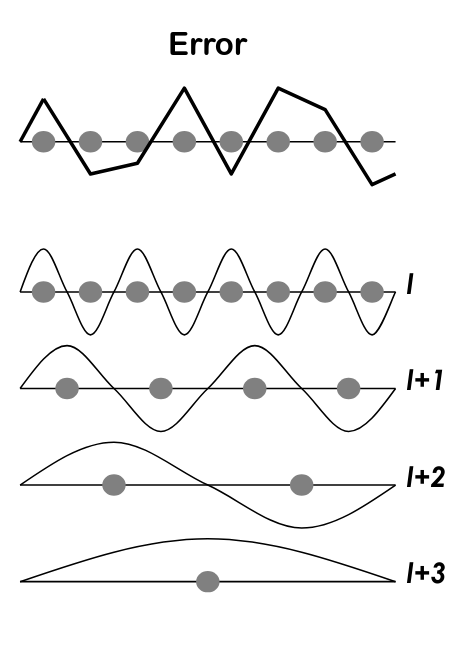
\includegraphics[width=\linewidth]{figures/Literature review/multigrid.png}
\vspace{-2em}
    \caption{Multigrid error prolongation over various mesh spacings \cite{ModestiHickel2025CFDslides}}
\vspace{-0.5em}
    \label{fig: multigrid}
\end{wrapfigure}

Multigrid is a technique in which the conventional iterative procedure is combined with a correction of the solution on a sequence of coarser meshes. These methods accelerate the solution of linear (and non-linear) systems by applying a direct solving algorithm to the system on various levels of grid resolution \cite{Driss2018}. Because solving algorithms (like Gauss-Seidel) are efficient at removing small-frequency wave lengths from the error distribution, but not at removing significant frequency errors, multigrid maps these larger frequencies to coarse meshes such that they appear smaller to the solver and will thus be more quickly resolved.  

Multigrid is usually implemented over a grid hierarchy, where the algorithm cycles to progressively coarser grids to ensure faster convergence. The pattern the algorithm takes can take various forms, where the most often used paths are described by the V and W cycle \cite{Driss2018}. Modern CFD solvers employ these multilevel multigrid methods in two distinct ways: geometric multigrid (GMG), where coarse levels are generated by reducing the resolution of the structured computational grid, and algebraic multigrid (AMG), where the hierarchy is constructed directly from the system matrix. AMG is particularly advantageous for unstructured meshes, where matrix connections lack a regular geometric pattern \cite{Driss2018}. Using this recursive implementation, multigrid methods typically approach $\mathcal{O}(N)$ or $\mathcal{O}(N \: log \, N)$ scaling, where N is the number of grid points \cite{Germaschewski2005}. Because of this property, multigrid methods are often described as having "optimal time complexity" \cite{Lhner2013}.

This method has shown promising results for LES, where \textcite{Gravemeier2010} has demonstrated that a purely algebraic variational multigrid can improve scale separation in LES. This, in turn, led to more accurate simulations for a reduced computational cost. 

Multigrid methods are one of the various methods that can be used to accelerate the convergence of ill-posed linear (or nonlinear) systems using an iterative solver. It is part of a collection of so-called preconditioning schemes, which are methods for making ill-conditioned or stiff matrix equations converge more quickly. More popular preconditioning schemes are the ones postulated by \textcite{Turkel1999}, \textcite{Weiss1994}, \textcite{Meijerink1977} and \textcite{Chapman2000}.

\subsubsection{Alternative time stepping}
Alternative time stepping is a method used in CFD solvers to improve convergence rates and stability by adjusting the time stepping scheme employed by the solver. Explicit time-stepping schemes, such as the forward Euler method, are particularly dependent on the Courant-Friedrichs-Lewy (CFL) number to maintain stability. The CFL number is influenced by the time step size chosen by the solver and is inversely related to the grid spacing. This means that in a constant time stepping scheme, the smallest grid cell dictates the system's stability.

To solve this issue, the time step can be adapted throughout the simulation. This is achieved by monitoring the solver's convergence and adjusting the time step to either ensure convergence or accelerate it. The most recent advances in Adaptive Time Stepping (ATS) have shown promising results when coupled with an implicit time integration scheme on false transient RANS schemes \cite{Nived2025}. In false transient RANS, the time evolution is treated as a computational artefact, referred to as "pseudo-time," rather than a physically accurate temporal progression \cite{Nived2025}. ATS has also been successfully applied to various turbulent flow cases, such as incompressible flow over a flat plate, the NACA-0012 airfoil, and various aircraft wings \cite{Nived2025}. Where they have shown significant decreases in computational cost, using explicit time integration with adaptive time stepping is almost crucial; otherwise, computational time could be unnecessarily prolonged or become unstable. 

Another way to increase the convergence rate by applying an alternative time-stepping scheme is to use local time stepping (LTS). LTS aims to minimise the global CFL restrictions by allowing different parts of the computational domain to use different time steps based on the local CFL requirement \cite{Esnault2010}. This approach is beneficial for simulations where certain regions require finer resolution than others, such as the inflow compared to the boundary layer of an airfoil. This situation typically creates meshes with a wide range of different cell sizes, and thus, the global CFL number is bounded by the smaller cells. LTS can generally be categorised into hierarchical and non-hierarchical approaches. Hierarchical methods employ techniques such as Adaptive Mesh Refinement (AMR), which will be discussed later in this document, to apply different time steps to different parts of the domain. Non-hierarchical methods focus on creating an interface between neighbouring grids that utilise different time steps \cite{Esnault2010}.

Multigrid and alternative methods are just a few ways in which convergence can be stabilised or improved; numerous other methods achieve the same goal, which will not be listed in this literature review (see \cite{Nived2025, vermeire2013, Esnault2010, Kalkote2019, Sreejith2022} and the references therein). 


% \subsection{Reduced Order Modelling}
% \label{subsect: reducedordermodelling}
% Reduced Order Models (ROMs) are methods which are designed to accelerate unsteady CFD simulations by replacing the original model, the NSE, with a lower-order model that can still accurately describe the essential phenomena of the flow. ROMs are low-order models derived from an appropriate projection of the full system's degrees of freedom (DOF) to a much smaller amount of DOF that is still able to encapsulate most of the system's fundamental dynamics\cite{Lucia2004}. The most popular way to derive a ROM is by applying Proper Orthogonal Decomposition (POD).

% \subsubsection{Proper Orthogonal Decomposition}
% Proper Orthogonal Decomposition or POD for short, is used in CFD to split a time dependant flow field $u(x, t)$ into time independent orthonormal basis functions $\varphi(x)$ and time dependant orthogonal coefficients $\alpha(t)$ \cite{Cizmas2008}. To do this a simulation of the full order model of $u(x, t)$ needs to be calculated first, of which M snapshots have to be taken at various time instances to form a snapshot matrix of the flow field, such that: $u(x, t_i), i=1,...,M$ \cite{Cizmas2008}. After the snapshots have been collected, the aforementioned basis functions are extracted by applying Singular Value Decomposition (SVD) to the snapshot matrix. After having completed the SVD the eigenvectors associated with the largest eigenvalues are selected, as they capture the modes with the highest amount of energy or largest flow features. 

% \begin{figure}[h]
%     \centering
%     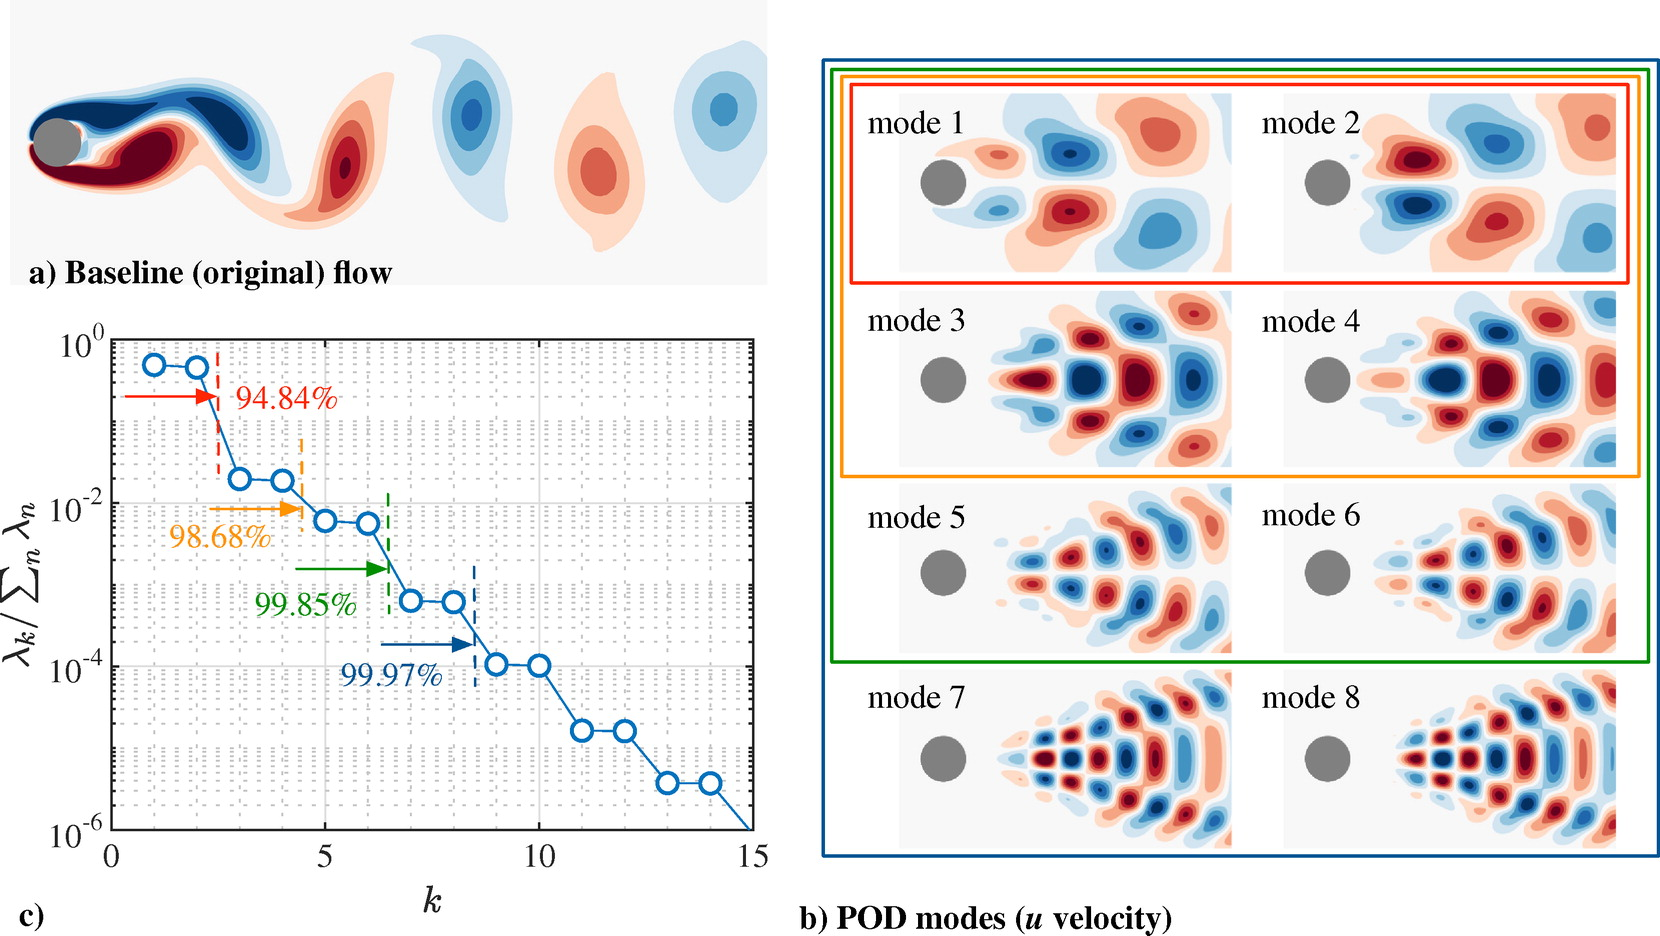
\includegraphics[width=0.75\linewidth]{figures/Literature review/POD.jpeg}
%     \caption{POD analysis of cylinder flow: a) original flowfield under study (vorticity shown), b) first eight dominant POD modes, and c) amount of KE of unsteadiness captured by the POD modes. Adapted from \cite{POD}}
%     \label{fig: POD}
% \end{figure}

% As seen in \autoref{fig: POD}, the first few modes capture the bulk of the flow's energy, indicating that with a limited amount of modes over 95\% of the energy in the system can be represented in the ROM. The left side of \autoref{fig: POD} shows the spatial modes of the velocity field, revealing the characteristics of the alternating vortices. These modes can be used in a linear combination to reconstruct or approximate the original flow field:

% \begin{equation}\label{eq: POD}
% u(x, t_i) = \sum_{k=1}^{M} \alpha_k(t_i) \, \varphi_k(x), \quad i = 1, \dots, M,
% \end{equation}

% Where the right hand side of \autoref{eq: POD} is a an approximation of the original higher order flow field. To determine the unknown time dependant coefficients $\alpha(t_i)$ \autoref{eq: POD} is projected onto the POD basis of the NSE using a Galerkin projection \cite{Lucia2004}. Which leaves us with a set of low order equations where the degrees of freedom depend on the amount of modes which were used in the reconstruction and the accuracy of the ROM depends on the amount of snapshots used when making the snapshot matrix. 


% Because of this reduction in degrees of freedom the computational cost goes down drastically. As the work of \textcite{Lucia2004} showed that a full order model of 64400 DOF's could be reduced to 8 DOF's which managed to speed a simulation of 6.2h up to just 8.1 seconds while maintaining a stable and accurate solution. Similarly \textcite{Ripepi2018} showed that a mesh a mesh around an LANN wing with 450,560 elements could be reduced to a ROM using 17 POD modes reduced the amount of solver iterations by 50\% and achieved a speed up of 38\%. Both of these cases show the power of implementing ROMs for CFD acceleration. 

% Beyond POD there are other approaches for reducing complexity of turbulent flow simulations. Methods like Volterra theory, Harmonic balance or using the snapshots of the higher order simulation as basis vectors. These are however left outside the scope of this literature review, the works by \cite{Djeddi2017, Cizmas2008, Lieu2006}, and the references therein, offer further insights in these other approaches.

% There are however drawbacks to these methods, firstly to create the ROM a preliminary simulation needs to be ran to obtain the snapshot matrix. This requires a significant amount computational cost, which is exactly what ROM's are trying to avoid. Secondly, the accuracy of the ROM is highly dependant on the quality of the snapshots used in the snapshot matrix. Meaning that if snapshots are taken at time intervals were certain flow phenomena are not present, they will also not be present in the POD modes. Which will in turn mean that they will also not be present in the ROM, leading to a decreased accuracy of the ROM. Lastly, POD based ROM's are susceptible to a lack of robustness to changes in the parameters that govern the system behaviour\cite{Lucia2004}. Meaning that if you would want to test an airfoil over various angles of attack with POD based ROMs, every angle of attack would need its own snapshot matrix and have SVD applied again, which is just as time consuming as running the higher order model. 


\subsection{Mesh and model adaptations}
\label{subsect: meshandmodel}
Alongside alternative numerical and algorithmic techniques, simulations can also be accelerated by making mesh and/or model adaptations that can reduce computational costs. This subsection will discuss the various ways in which model adaptations and combinations have been accelerating CFD simulations.

\subsubsection{Adaptive Mesh Refinement} 
Adaptive Mesh Refinement (AMR) is a framework that dynamically adjusts the mesh resolution of the computational domain based on the evolution of the solution. Initially developed for the numerical solution of hyperbolic partial differential equations \textcite{Berger1984} and later improved for conservation laws in \textcite{Berger1989}, where AMR was used to efficiently resolve shockwaves in the solution, while limiting computational costs. AMR is beneficial for problems where physical length scales vary significantly across, or when complex features like shockwaves present themselves in the flow. 

\begin{figure}[h]
    \centering
    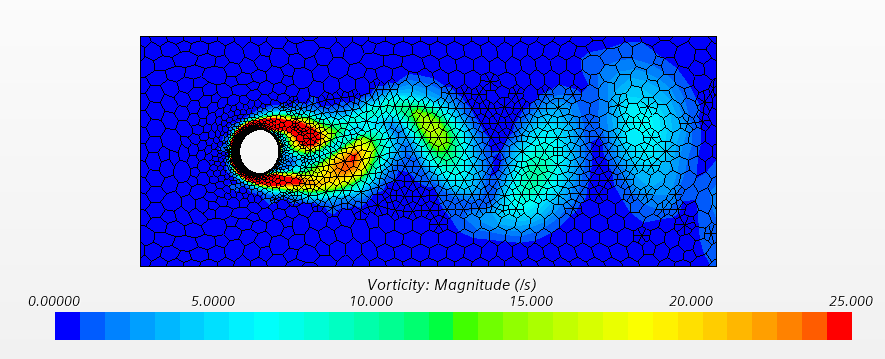
\includegraphics[width=\linewidth]{figures/Literature review/FlowOverCylinder.png}
    \caption{AMR being applied over the wake of a cylinder experiencing vortex shedding in its wake. Adapted from \cite{starcyl}}
    \label{fig: FlowoverCyil}
\end{figure}

AMR employs a hierarchical grid system where the domain is first discretised with a coarse 'parent' mesh. Regions that require higher resolution are subsequently covered with a finer 'child mesh'. These finer child meshes will then also use a smaller time step than those of the parent mesh. This connects AMR to the ATS scheme explained previously. After this, the truncation error is assessed at each cell to determine where mesh refinement is needed \cite{Berger1984}. If the truncation error of a specific cell exceeds the desired level, the grid is refined in this region. The algorithm then attempts to minimise overlap and limit the number of patches refined. On the other hand, cells which are no longer required to be refined can be dropped to save on computational cost. \autoref{fig: FlowoverCyil} shows how AMR is being executed in the wake of the cylinder to capture the coherent structures being formed due to vortex shedding. 

Applying AMR leads to a decrease in computational cost, as the dynamic control of the total number of cells minimises computing time while maximising solution accuracy by providing a highly resolved solution only where required. That is why AMR has become the method of choice, while in others, a technique of necessity, for fields like astrophysics and combustion \cite{plewa2005}. One example of AMR is \textcite{Shahsavan2018}, where AMR was used to investigate whether replacing nitrogen with argon in the intake mixture enhances the auto-ignition and combustion characteristics of combustion engines. Because of its fullness, various frameworks have also been developed to make AMR available to a broader public \cite{Dubey2014, MacNeice2000}
 
\subsubsection{Wall models}
Wall models are a crucial component for turbulent flow simulations, particularly for LES of wall-bounded flows. The computational cost of fully resolving the near-wall region is prohibitively expensive at high Reynolds numbers. Where the total work of determining the inner layer of the boundary layer scales with approximately $Re^{2.4}$\cite{LARSSON2016}. Wall models address this issue by modelling the effects of the innermost layer of the boundary layer on the resolved scales, which significantly reduces computational costs. 

Wall models generally operate by replacing the traditional no-slip boundary condition at the wall by a modified stress boundary \cite{Piomelli2008}. They can usually be categorised into two distinct groups: wall stress models and hybrid LES/RANS \cite{LARSSON2016}. Wall stress models are based on the principle of energy conservation in a near parallel shear flow \cite{LARSSON2016}, meaning that the wall model aims to model the wall shear stress $\tau_{wall}$ by utilising the RANS boundary layer equation in \autoref{eq: wallmodel} 

\begin{equation}\label{eq: wallmodel}
\frac{\partial \overline{u}_i}{\partial t}
+ \overline{u}_j \frac{\partial \overline{u}_i}{\partial x_j}
+ \frac{1}{\rho} \frac{\partial p}{\partial x}
= \frac{\partial}{\partial y} \left[
\left( \nu + \nu_{t,\mathrm{wm}} \right)
\frac{\partial \overline{u}}{\partial y}
\right]
\end{equation}

The most common wall stress model is the equilibrium model, in which the convection and the pressure gradient balance each other out. This means that the left-hand side of \autoref{eq: wallmodel} is assumed to be zero. This leads to an ODE that, when using mixing length theory, has a solution in the form of $u^+ \approx y^+ \quad\text{for } y^+ \lesssim 5 \quad \text{and} \quad u^+ \approx \frac{\ln(y^+)}{\kappa} + B \quad \text{for } y^+ \gtrsim 30$, which is the model used for the algebraic wall stress model \cite{LARSSON2016}. By implementing these solutions, the equilibrium model, and all other wall stress models, aim to match the velocity profile seen in \ref{fig: lawofthewall} 

\begin{figure}[H]
    \centering
    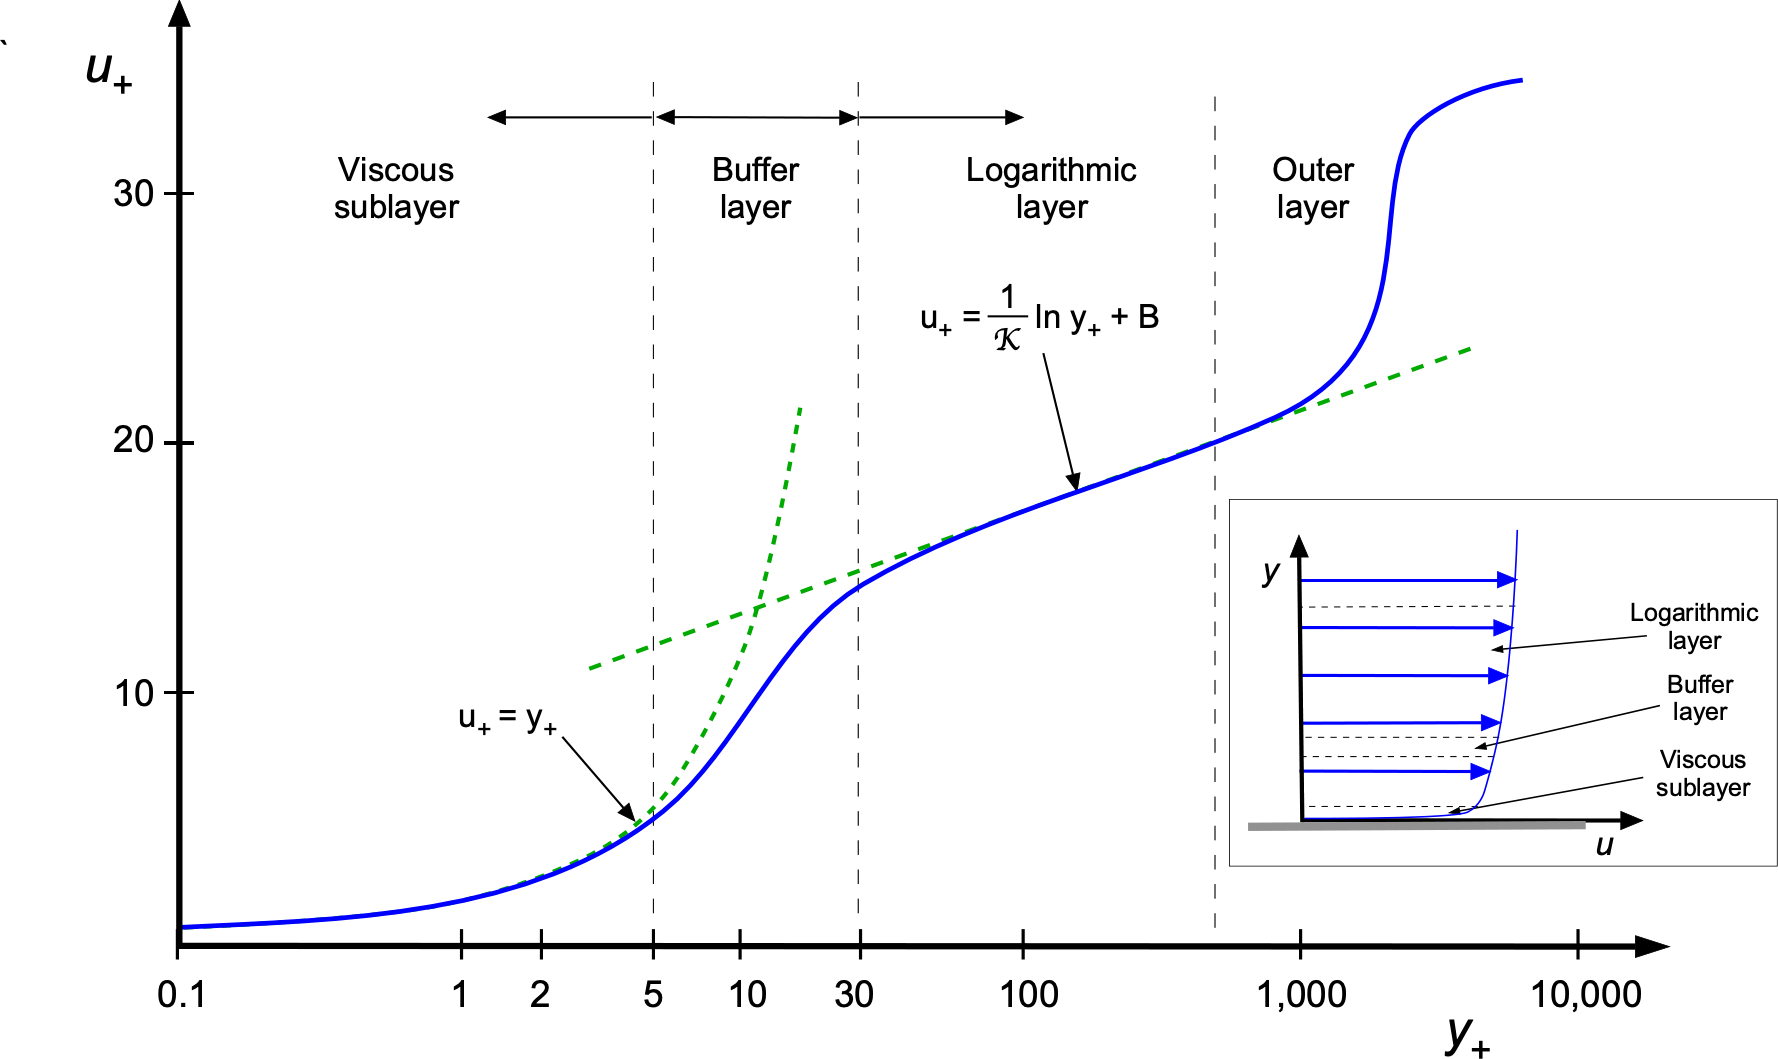
\includegraphics[width=.7\linewidth]{figures//Literature review/wall_law.png}
    \caption{Velocity profile $u+$ vs. $y+$ showing the viscous sublayer, buffer layer, and log-law region. The linear and logarithmic approximations (dotted) are compared to the full profile (blue). Adapted from \cite{Leishman2023}}
    \label{fig: lawofthewall}
\end{figure}


Another way to model the near-wall region is to resolve the left-hand side of \autoref{eq: wallmodel} locally, which leads to a more complex $\nu_t$. This ODE approach \cite{LARSSON2016} enables a more realistic wall model, but it does lead to higher computational costs. More advanced wall stress models have been proposed by \textcite{Hickel2015} and the references therein, which aim to incorporate non-equilibrium effects to predict flow separation better.

The other class of wall models are the hybrid RANS/LES models, where the idea is to apply a RANS approach to modelling the inner part of the turbulent boundary layer and an LES-type subgrid model to the outer layer \ cite {Hickel2015}. These can essentially be divided into zonal methods and blended methods. Where the former separate RANS and LES computations with a set interface, which can be fixed by the user or dynamically adjusted by the solver, as was proposed in the work of \textcite{Qumr2002}. In contrast, blended methods switch between RANS and LES modes in a way that cannot be set by the user, with the most famous example being the Detached Eddy Simulation (DES). A good overview of these various wall models is presented in the work of \textcite{LARSSON2016}.

\subsection{Parallelization techniques}
Besides adaptations to meshing, time integration, numerical algorithms and modelling approaches, computational cost can be lowered through the strategic application of parallel computing architecture, utilising both CPU (Central Processing Unit) and GPU (Graphics Processing Unit) computation power. This approach is fundamental for handling the increasingly rising computational demands of complex turbulent flows and large-scale industrial or research problems \cite{Driss2018}.
Parallel computing or parallelisation is the simultaneous execution of multiple computational tasks on a multiprocessor system by distributing the computational load among the different processors \cite{Afzal2017}. By executing numerous tasks on various processing units, large tasks can be completed more quickly. In previous decades, performance gains in scientific computing were achieved through breakthroughs in hardware engineering, such as an increase in clock speed or lithographic advancements. However, as \textcite{Shalf2020} indicated, the era of continuous performance gains has ended, partly due to limitations in clock speed scaling (due to excessive power consumption) and the increase in transistor density approaching physical limitations. This means that to ensure accelerations in the near future, architectural advances will be the most practical path to continue the growth of high fidelity CFD applications\cite{Shalf2020}. This subsection highlights key parallel computing strategies that have been developed over time. 


\subsubsection{OpenMP}
Open Multi-Processing (OpenMP) is a widely adopted parallelisation tool which enables computations to be distributed across multiple threads running on the cores of a single processor or within a single shared memory system \cite{Afzal2017}. OpenMP's leading role in CFD is to enable parallel execution without requiring the decomposition of the computational domain or communication between processes, as all threads operate within the same memory space. Since the computational grid does not need to be subdivided into smaller subdomains, there is no need for communication between processes, which reduces the total computational cost of the algorithm and simplifies load balancing\cite{Afzal2017}. Due to its flexibility and ease of path development, OpenMP is supported by virtually all major compiler vendors. Making it a popular choice for enabling internal node parallelism. 

The work of \textcite{Afzal2017} listed various examples of parallelisation of CFD codes using OpenMP. As his work is already quite extensive, this literature review will not provide examples of OpenMP implementation. 

In the context of high-fidelity CFD applications, OpenMP does offer some disadvantages. These mainly arise from its limited scalability, due to its restriction to shared memory architectures, which means it struggles with enormous CFD problems that are difficult to load into a single memory cache \cite{Afzal2017}. For these significant CFD challenges, OpenMP is often deployed in a hybrid approach alongside tools like MPI, where it handles the parallel work on the cores within each node. This complements the role of MPI in coordinating computations across separate nodes. MPI and this hybrid model, along with their applications, will be explained further in this subsection. 

\pagebreak
\subsubsection{MPI}

\begin{wrapfigure}{r}{0.5\linewidth}
% \vspace{-4em}
    \centering
    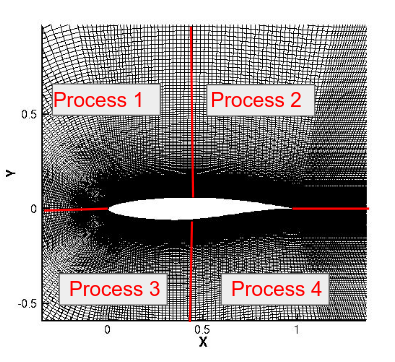
\includegraphics[width=\linewidth]{figures//Literature review/MPI_decompose.png}
    \caption{Decomposition of the computational domain around an airfoil across four different nodes \cite{ModestiHickel2025CFDslides}}
    \label{fig: MPImesh}
    \vspace{-1em}
\end{wrapfigure}

Message Passing Interface (MPI) is also a key standard for parallelisation on distributed memory platforms. It provides a collection of commands which exchange messages and manage processes between processing units. Unlike OpenMP, which is designed for shared memory systems where all parts of the program can access the same data in a single memory pool, MPI is used for distributed memory systems, where each processing unit has its own private memory \cite{Giovannini2015}. In the context of CFD, engineers often deal with vast computational domains that require extensive amounts of memory and processing power. Where using a single memory cache or processing unit would not be fast enough to solve these types of problems on its own. MPI allows the user to distribute these significant problems across many different nodes, where each node has its own private memory that the other nodes can't access. Each node (which can be a processor core or an entirely different computer) works on a portion of the overall simulation. 

To ensure the overall CFD solution is accurate and continuous, the sub-domains need to exchange information at their boundaries; MPI provides the communication protocol for this exchange. In CFD, data is exchanged for "ghost cells" or "halo cells" which are at the interface between neighbouring sub-domains. These cells contain data from adjacent blocks that a processor unit needs to correctly calculate its own part of the solution \cite{Afzal2017, Giovannini2015}. An example of this mesh decomposition can be seen in \autoref{fig: MPImesh}, where MPI ensures that processes 2 and 4 receive the correct flow information from processes 1 and 3, respectively. 


\textcite{Afzal2017} reported various implementations of the MPI protocol, which achieved significant CFD speed-up results. These results generally follow the trends predicted by Amdahl’s law \cite{Amdahl1967}, which, for CFD applications, limits the maximum theoretical speed-up to around 20x. However, Amdahl’s law is only a theoretical bound; in practice, MPI implementations in CFD often achieve better scalability due to improved algorithms, communication strategies, and domain decomposition \cite{Giovannini2015, Hadade2016}.


% \begin{wrapfigure}{r}{0.5\linewidth}
% \vspace{-2em}
%     \centering
%     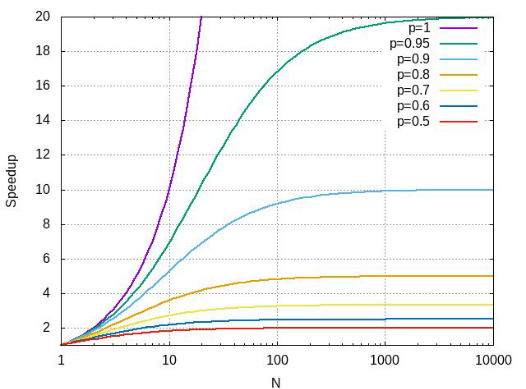
\includegraphics[width=\linewidth]{figures//Literature review/Amdahl.png}
%     \caption{Amdahl's law: Theoretical speed-up as a function of the number of processors $N$ for different parallel fractions $p$. The speed-up saturates as $N$ increases due to the serial portion $s = 1 - p$ of the workload \cite{ModestiHickel2025CFDslides}}
% \label{fig: Amdahl}
% \vspace{-1em}
% \end{wrapfigure}

% Again \textcite{Afzal2017} indicated various implementations of the MPI protocol, which achieve significant CFD speed-up results. These speed-ups generally follow the theoretical limits described by Amdahl's law \cite{Amdahl1967}, which is a formulation that explains how much faster a task can be completed for a fixed workload when more computational resources are added to the system. Amdahl's law states that the achievable speed-up is limited by the fraction of the code that must remain serial, as shown in \autoref{fig: Amdahl}. Even with an increasing number of processors, the achieved speed-up levels out unless nearly all operations can be parallelised.

% \begin{equation}\label{eq: Amdahl}
%     \text{Speedup}=\frac{1}{s + \frac{p}{N}}
% \end{equation}

% \autoref{eq: Amdahl} shows the formula that governs Amdahl's law, where $p$ is the fraction of processes that can be parallelised, $N$ is the number of processing units, and $s$ (which is equal to $1-p$) is the fraction of processes which can not be parallelized \cite{Hill2008}. Since CFD applications can be parallelised using MPI, they generally have a high parallel fraction of $p\approx0.95$. When following Amdahl's in \autoref{fig: Amdahl}, this parallel fraction allows a 20 times speed up compared to single core execution. This limit is, however, an example, and literature has shown better parallel fractions\cite{Giovannini2015, Hadade2016}.

\subsubsection{CUDA}

\begin{wrapfigure}{r}{0.5\linewidth}
\vspace{-1em}
    \centering
    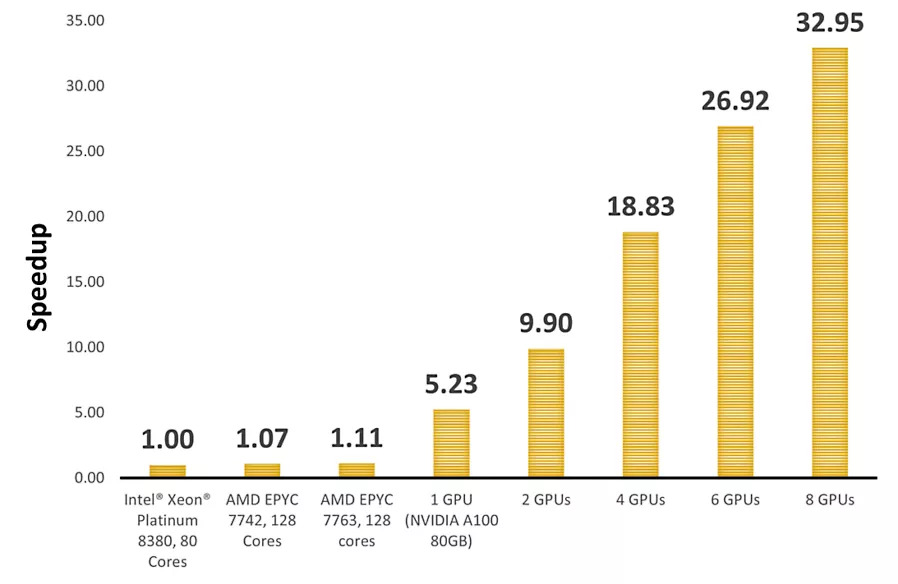
\includegraphics[width=\linewidth]{figures/Literature review/GPU.jpg}
    \caption{Speedup comparison of CFD simulations across CPU and GPU hardware configurations. The results show modest gains with CPU alone, while GPUs offer significant performance improvements. Adapted from \textcite{ansys2023multiGPU}}
\label{fig: GPU}
\vspace{-1em}
\end{wrapfigure}

Due to advances in GPUs, the Compute Unified Device Architecture (CUDA) stands out as a prominent framework for leveraging GPUs to achieve significant computational speed-ups. CUDA, a platform developed by NVIDIA, provides a general-purpose parallel computing platform specifically designed for their GPU architectures \cite{Lai2020}. When implemented, CUDA allows CFD solvers to employ the massive computational power and high memory bandwidth of the GPU, where it acts as a 'co-processor' to the CPU. The CPU, or "host," handles the sequential parts of the application and overall control logic, while the GPU, or "device," takes on the massively parallel computational tasks \cite{Xiang2017}. 

 CUDA has enabled CFD researchers to achieve speedups of over 50\% compared to the sequential CPU version, as demonstrated in the work of \textcite{Lai2020}. The authors benchmarked two commercially available GPUs for the HSMAC (Highly Simplified Marker and Cell) and SIMPLE (Semi-Implicit Method for Pressure-Linked Equations) algorithms in a 2D Lid-Driven Cavity Flow. GPUs allow a more cost-effective solution for parallel computing than expensive CPU clusters, making high-performance computing more accessible to researchers \cite{Chen2009}. The work of \textcite{Afzal2017} illustrates more examples of CUDA parallelisation and computational speed improvements, which will not be discussed in this work as the primary focus lies on accelerating high-fidelity CFD cases. \textcite{ansys2023multiGPU} has also demonstrated that one NVIDIA A100 GPU outperforms a HPC cluster with 400 Intel Xeon Platinum 8380 cores, while doing so for up to 7 times cheaper hardware costs. 

 Furthermore, GPU devices offer a more cost-effective and energy-efficient solution compared to expensive CPU clusters \cite{Afzal2017}. This ties back to the statement made earlier in this section, where clock speed advancements have to be limited due to high power demands.  

While GPU acceleration through CUDA represents a powerful avenue for enhancing solver performance, especially for large-scale unsteady simulations, its integration often requires significant code restructuring and hardware-specific modifications \cite{Afzal2017}. Due to the large computational domain of high-fidelity CFD cases, such as LES, memory transfer between the CPU and GPU can present itself as a significant bottleneck in CUDA implementations. This is due to the considerably slow transfer speed over the CPU-GPU connection compared to the GPU's internal memory bandwidth \cite{Xiang2017, Afzal2017}. 

\subsubsection{Hybrid parallelization methods}
Knowing the strengths and weaknesses of OpenMP, MPI, and CUDA has motivated researchers to combine these methods into hybrid parallelisation frameworks, which aim to leverage the strengths of each of these methods. As mentioned before, MPI is well-suited for distributed memory systems and decomposition of large CFD fields, while OpenMP is utilised in finer parallelisation tasks. One example of OpenMP and MPI being combined is the work of \textcite{Jin2011}, where MPI is used for communication across distributed memory nodes and OpenMP is used for fine-grained parallelisation within the node \cite{Jin2011}. The work demonstrated that the combination of OpenMP and MPI yielded the best results when fewer MPI tasks were performed with moderate OpenMP threading. 

OpenMP and CUDA have also been combined to leverage each other's strengths. The work of \textcite{Yue2014} leveraged these methods in a way that the parts that could not be parallelised over the GPU were parallelised by the CPU using OpenMP. Furthermore, optimisation of different types of memory was achieved by using shared memory to decrease latency between the GPU threads, thus promoting overall performance \cite{Afzal2017}.

The combination of MPI and CUDA is a popular strategy for HPC clusters, combining the memory parallelism between nodes deliverable by MPI with the massive memory and computing power of GPUs. Similar to the OpenMP and CUDA hybrid method. The method implemented by \textcite{Lai2020} uses the CPU to manage the GPU execution and communication. At the same time, the GPU performs the primary data processing,  which has shown significant improvements compared to CPU executions. Furthermore, the study by \textcite{Jacobsen2010} has also indicated the significant speed-ups that MPI-CUDA parallelisation can deliver in GPU HPC clusters, showing speed-ups of more than 100\% for 128 GPUs \cite{Jacobsen2010}.

\subsubsection{Future Outlook and Current Bottlenecks}
As previously mentioned, the future of using hardware to achieve accelerated CFD simulations is shaped by the end of the traditional processor scaling (Moore's law \cite{moore1965}) and an ever-growing need for more complex flow simulations, which is why companies like NVIDIA are enabling significant advancements in architectural specialisation. \textcite{Shalf2020} predicts that a shift towards architectural specialisation is needed, as HPC platforms become increasingly heterogeneous. That is why one way of ensuring continued performance improvements is to use transistors more efficiently by specialising the architecture to the target scientific problem \cite{Shalf2020}.

Due to the increasing complexity and size of CFD domains, data movement is presenting itself as a bottleneck in performance. Due to the vast amounts of data that need to be handled by the hardware architecture, the energy required to move data exceeds the energy used to process that data \cite{Shalf2020}. On the other hand, these vast amounts of data present a unique opportunity. The large amount of data generated from high-fidelity CFD cases can be leveraged to develop data-driven acceleration schemes that approximate flow or surrogate models, replacing the computationally expensive parts of the solver. This is where machine learning and artificial intelligence techniques might find their place in the industry. These models can be trained on these large amounts of data to accelerate and can provide interesting predictions or optimised acceleration techniques. This way, the very data that seems to be a bottleneck to hardware acceleration schemes can enable interesting new CFD acceleration strategies, which will be explained in the rest of \autoref{sect: 2.5ML enhancing}

\section{Machine/Deep learning Enhanced CFD}
\label{sect: 2.5ML enhancing}
The integration of machine learning (ML) into the CFD field presents interesting opportunities for acceleration frameworks for turbulent flow simulations. Where traditional performance-enhancing methods in \autoref{sect: 2.4performance enhancing} can offer significant performance gains, they remain constrained by their reliance on numerical algorithms. This is where data-driven methods can complement these traditional methods by leveraging the massive amounts of available high-fidelity simulation data. 

\begin{wrapfigure}{l}{0.5\linewidth}
    \centering
    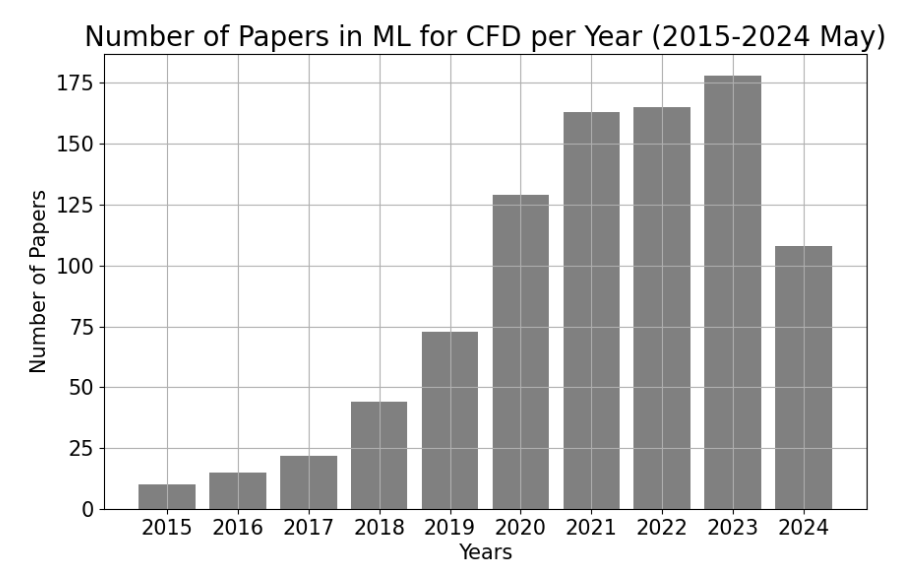
\includegraphics[width=\linewidth]{figures//Literature review/MLpapers.png}
    \caption{Rise in the amount of ML papers in CFD \cite{Wang2024}}
    \label{fig: MLPapers}
    \vspace{-1em}
\end{wrapfigure}

It is worth noting that recent years have seen an exponential growth in the number of studies exploring ML-enhanced CFD. Countless methods incorporating ML into the CFD landscape have been developed, ranging from broadly adopted to more niche applications. Comprehensive reviews, such as those by \textcite{Vinuesa2022} and \textcite{Wang2024}, demonstrate the rapid advancements in the field. \autoref{fig: MLPapers} visualises this trend, showing how the number of papers on ML for CFD has shown a steady increase in the last 5 years. Given the sheer volume of available material, it is beyond the scope of this work to cover all relevant contributions in detail.

% Instead, this section will highlight core ML and DL concepts, with selected CFD-acceleration frameworks that align with the central research question posed in \autoref{chap: Introduction}.

Before highlighting the current landscape of ML-enhanced CFD simulations, \autoref{subsect: intro to ML} and \autoref{subsect: introtoNN} will briefly handle ML and NN terminology before \autoref{subsect: commonNN} will introduce key neural network architectures which are frequently used in the CFD environment. Where \autoref{subsect: PIsurrogates}, \autoref{subsect: data driven ROMS}, and \ref{subsection: ML solver} will showcase how ML can be leveraged to accelerate CFD simulations by enhancing solver components, employing data-driven ROMS and creating physics-informed surrogate models. 


\subsection{Introduction to Machine Learning}
\label{subsect: intro to ML}
Machine Learning is a branch of artificial intelligence that aims to develop algorithms capable of learning patterns and making predictions from data without being explicitly programmed. ML models can essentially be expressed as a function $\boldsymbol{y}(\boldsymbol{x})$ which takes an input vector $\boldsymbol{x}$ and transforms it to an output vector $\boldsymbol{y}$. The precise form of $\boldsymbol{y}(\boldsymbol{x})$ is determined during the \textit{training phase} based on the training data \cite{bishop2007}. The training of the model requires a dataset that is usually split into training, validation and test sets. The training set is used to fit the model parameters, while the validation set can be used to determine hyperparameters, such as the learning rate and network architecture. The test set evaluates the model's generalisation to unseen data \cite{burkov2020}. 

Depending on the target variable, ML objectives are typically categorised into two categories: regression (continuous outputs such as velocity or pressure predictions) and classifications (discrete categories, e.g., image recognition and Optical Character Recognition).

A central challenge in ML is ensuring that models generalise beyond the training data, meaning that they can reliably generate correct outputs for unseen data that was not in their training set. Overfitting occurs when a model has been trained to achieve an extremely high accuracy on the training data, resulting in poor predictions on unseen test data. While underfitting reflects a model that is too simple to capture the underlying dynamics of the training data, resulting in poor performance even on the training data \cite{burkov2020}. To address these pitfalls, regularisation strategies, careful dataset design, and physically informed constraints can be employed to reduce model complexity and penalise unrealistic predictions \cite{Aggarwal2018, sanderse2024}.

ML algorithms are broadly grouped into three categories: supervised learning, where models learn from labeled data (most common in CFD, like mapping flow fields to forces); unsupervised learning, which identifies patterns or reduced representations from unlabelled data (e.g., clustering coherent flow structures or dimensionality reduction); and reinforcement learning, where an agent interacts with an environment to optimize a reward. 

A detailed treatment of machine learning theory is beyond the scope of this work. Still, it can be found in standard references such as \textcite{bishop2007, burkov2020, danie2021}, which provide the broader theoretical background underlying the CFD-oriented applications discussed further down in this work.

\subsection{Introduction to Neural Networks}
\label{subsect: introtoNN}

\begin{wrapfigure}{r}{0.5\linewidth}
    \centering
    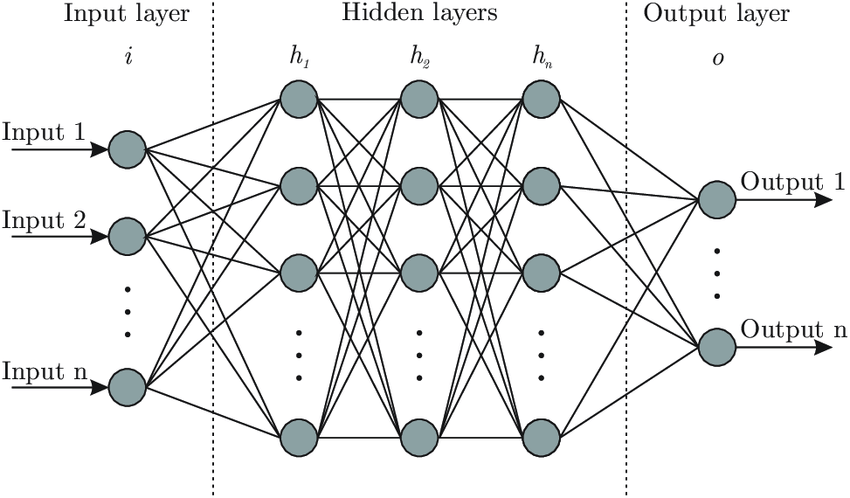
\includegraphics[width=0.8\linewidth]{figures/Literature review/NeuralNetwork.png}
    \caption{General architecture of a Feed Forward Neural network, adapted from \cite{nashtech_activation2023}}
    \label{fig: FNN}
\end{wrapfigure}

Neural networks (NNs) are a class of ML models inspired by the biological nervous system, designed to approximate complex nonlinear functions. They consist of interconnected computational units, or neurons, which receive inputs, process them through an activation function and produce an output. A general architecture of a NN can be seen in \autoref{fig: FNN}. The use of non-linear activation functions enables NNs to act as universal function approximators \cite{Hornik1989}, capable of representing highly complex mappings between inputs and outputs. 

Training a neural network involves minimising a loss function that quantifies the difference between predictions and actual values across the dataset. This optimisation is typically performed through gradient descent and its variants, with gradients computed efficiently using the backpropagation algorithm \cite{Aggarwal2018}. To achieve a desirable accuracy, hyperparameters such as learning rate, network depth, and activation function can be optimised by monitoring the network's performance. After training is completed, a set of weights and biases is created that defines how the network transforms inputs into outputs.

The architecture of a NN can significantly affect its performance on different tasks. The simplest form of NNs are feed-forward neural networks (FNNs), as seen in \ref{fig: FNN}, where information flows from input to output in a single pass.

% where the NN displays an input layer on the left, hidden layers in the middle and an output layer on the right. A network where information flows follows this path is called a feed-forward neural network (FNN) \cite{Aggarwal2018}.

\subsection{Common Neural Network Architectures Employed in CFD}
\label{subsect: commonNN}

\subsubsection{Convolutional Neural Networks}
Convolutional Neural Networks (CNNs) are a frequently used class of neural networks specifically designed to process grid-structured input data that exhibit strong spatial dependencies in local regions of
the grid \cite{Aggarwal2018}. That is why CNNs are often used for image recognition, since adjacent spatial locations in an image often have similar colour values of the individual pixels. CNNs are characterised by convolution operations, which involve taking a dot product between a grid-structured set of weights (known as a filter or kernel) used to extract features from the input data.

Because of the strong capabilities of CNNs to extract features from image snapshots, they present
themselves as good candidates to be implemented for CFD predictions. Since CFD flow fields can
be represented as a structured grid, CNNs offer an outstanding possibility to learn patterns such as
vortices or boundary layers effectively. This can be helpful for tasks such as flow prediction, surrogate modelling, or acceleration \cite{Lee_You_2019, Guo2016}.


\subsubsection{Recurrent Neural Networks}

Recurrent Neural Networks (RRNs) are specifically designed for sequential data, where elements are ordered and depend on the value of the previous component of the series. Unlike traditional FFNs, RNNs take the inherent order of the data into account by processing inputs in sequence and treating them similarly relative to previous inputs. This behaviour is achieved by sharing the same set of network parameters across different temporal layers, allowing the network to maintain a hidden state that changes with each new input, effectively acting as a memory of past information \cite{Aggarwal2018}. 

However, RNNs often struggle to predict long-term dependencies due to the vanishing and exploding gradient problem, which can arise during training. To combat this, a variation of RNNs called Long Short-Term Memory (LSTM) networks addresses these issues by employing internal memory and gating mechanisms that regulate how information is stored, updated, or forgotten, allowing them to manage long-term dependencies more effectively. An overall structure of an LSTM is displayed in \autoref{fig: LSTM}, showing how the internal memory state $c_t$ refers to the work by \textcite{Aggarwal2018}, which provides an in-depth theoretical analysis of LSTMs, which are considered to be outside the scope of this literature review. For a more detailed explanation of RNNs, LSTMs, and the vanishing and exploding gradient problem, please refer to the work by \textcite{Aggarwal2018}, which provides an in-depth theoretical analysis of these concepts. 

\begin{figure}[h]
    \centering
    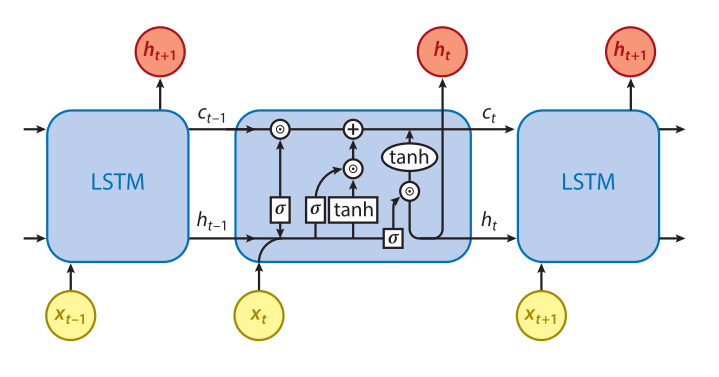
\includegraphics[width=0.75\linewidth]{figures//Literature review/LSTM.png}
    \caption{Structure of an LSTM cell with input, forget, and output gates regulating information flow through the memory cell. Source \cite{Brunton2020}}
    \label{fig: LSTM}
\end{figure}

LSTMs are particularly useful in CFD due to fluid dynamics being an inherently transient environment where time-dependent phenomena play a key role in accurate simulations. LSTMs generally excel at predicting temporal sequences and capturing complex non-linear dynamics over longer durations \cite{Aggarwal2018}. These capabilities have been demonstrated to be beneficial in enhancing CFD simulations and will be showcased later in this work. 


\subsubsection{Neural Ordinary Differential Equations}

Neural Ordinary Differential Equations (NODEs) are a type of deep neural network model introduced by \textcite{Chen2018} that differ substantially from conventional neural networks. They are similar to RNNs, and more specifically, Residual Neural Networks (ResNETs \cite{He2015}). In a ResNet, the latent space is represented by a stack of layers, as shown in \autoref{fig: ResNet}. NODEs learn the mapping of sequential data through a continuous representation of the latent space. 

\begin{wrapfigure}{r}{0.45\textwidth}
\vspace{-1em}
    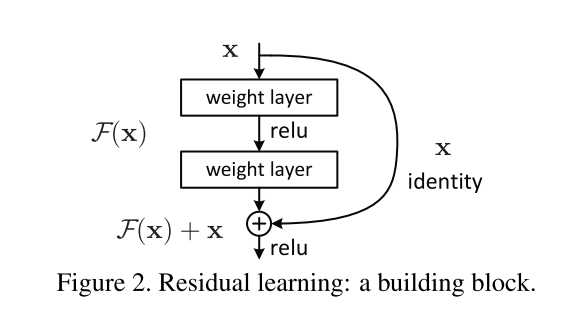
\includegraphics[width=1\linewidth]{figures//Literature review/ResNet.png}
    \caption{ResNet layer stacking, adapted from \cite{He2015}}
    \label{fig: ResNet}
% \vspace{-1em}
\end{wrapfigure}

Where the stacking of the latent state in ResNets can be seen as an Euler discretisation of a continuous transformation, shown in \autoref{eq: euler}

\begin{equation}\label{eq: euler}
    h_{t+1} = h_t + f(h_t, \theta_t)
\end{equation}

Where $h_{t+1}$ is the newly determined latent state, which is constructed of a summation of the current latent state $h_t$ through the addition of a function of the network parameters and value of the current prediction $f(h_t, \theta_t)$, when the added layers become large and the steps taken become smaller, this progression of the latent state can be represented by a differential equation \ref{eq: NODeODE}. 

\begin{equation}\label{eq: NODeODE}
   dh(t)/dt = f(h(t), t, \theta) 
\end{equation}

A conventional ODE solver can then be used to solve this equation. This formulation provides adaptive computation capabilities, as ODE solvers can dynamically adjust step sizes based on the solution's complexity, enabling an optimal trade-off between speed and accuracy. This essentially allows NODEs to define a smooth flow through the latent space, instead of a discrete series of transformations that ResNets produce. \autoref{fig: latentspace} shows a graphical representation of the latent space vector field.

\begin{wrapfigure}{r}{0.45\textwidth}
    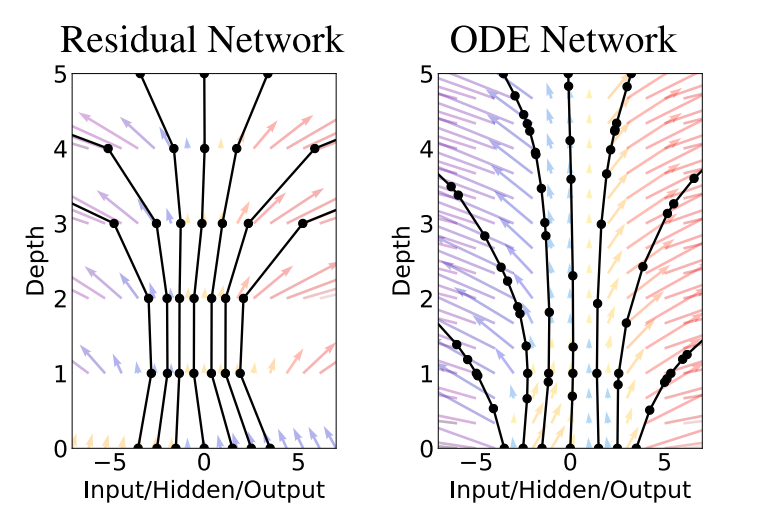
\includegraphics[width=1\linewidth]{figures//Literature review/latentspace.png}
    \caption{Left: Discrete evolution of ResNet predictions, Right: continuous evolution of predictions by NODE. Adapted from \cite{Chen2018}}
    \label{fig: latentspace}
\end{wrapfigure}

NODEs also provide a memory-efficient way to train deep models using the adjoint sensitivity method, which propagates through the ODE by solving a second augmented ODE backwards in time. Because the neural network can be viewed as a universal approximator, and the ODE solver can evaluate the latent layers at any time point for any timestep, the resulting model provides a smooth prediction without being constrained to discrete time steps or layers. This behaviour makes NODEs particularly well-suited for predicting systems where continuous time behaviour is essential, even if the supplied training data is irregularly sampled in time. 

In the context of CFD time-series prediction, NODEs can offer key advantages. Their adaptive behaviour can allow for variable time step integration, which can be optimal in accelerating potential CFD simulations. However, since NODEs involve solving ODEs and fluid systems are often high-dimensional, solving these ODEs can be computationally intensive. That is why, in recent literature, such as the work of \textcite{Shankar2022}, NODEs have been implemented within data-driven reduced-order models, where the dynamics of the latent space are predicted using NODEs. This aligns with the objective of this thesis, where instead of predicting the time integration of the NSE, the authors have implemented NODEs in the latent space of a ROM, which is used to predict the entirety of the latent dynamics, which can then be used as a surrogate model for a specific flow case. 

Another recent advancement in Neural ODE research has been the implementation of a physics-informed loss term. This embeds the governing equations of the system that the model aims to predict directly into the training process. \textcite{Sholokhov2023} introduced a collocation-based physics-informed loss function that enforces PDE constraints at sampled points, improving extrapolation, stability, and performance in situations where there is not a lot of training data available. Additionally, \textcite{Ghanem2025} proposed an optimisation framework that incorporates physics-informed loss terms, enabling the accurate recovery of hidden states when only partial measurements are available as training data. These works demonstrate that embedding physical laws into the NODE loss function allows for a more robust model in scenarios with sparse, noisy, or incomplete data. This type of approach could be particularly valuable in CFD, where enforcing conservation laws and physical consistency can lead to better flow field predictions using fewer training data. 

 
\subsection{Machine Learning Enhanced Solver Components}
\label{subsection: ML solver}

One way of leveraging ML to accelerate scale-resolved CFD simulations is by embedding machine learning directly into specific components of CFD solvers. Rather than learning the whole flow evolution, these approaches aim to improve the efficiency and accuracy of key solver stages. Calculations such as the Pressure-Poisson equation, RANS turbulence closure models, sub-grid scale models, or even learning-based discretisation are all possibilities that have been presented in recent literature. 

\subsubsection{Pressure-Poisson prediction}
As mentioned previously, an essential component of incompressible CFD solvers is the pressure-velocity coupling algorithm, which ensures that the computed velocity field remains divergence-free. This coupling is typically enforced in operator splitting methods to discretise the NSE, where first the velocity field is advected, and the resulting velocity field $\mathbf{u^*}$ does not satisfy the continuity equation \ref{eq: continuity}. This is then corrected using the Pressure-Poisson Equation (PPE) \ref{eq: PPE} \cite{Vinuesa2022}. 

\begin{equation}\label{eq: PPE}
    \frac{\Delta t}{\rho} \nabla^2 p = -\nabla \cdot \mathbf{u}^*
\end{equation}

Where $\Delta t$ is the simulation time step, $\rho$ the fluid density and $p$ the pressure field, finding the solution to this equation is typically the most computationally expensive for the numerical solver. This is why exploring alternative strategies for this computation could present promising acceleration results. 

\textcite{Chen2022} proposed a framework which employed a multi-scale Graph Neural Network (GNN) to either entirely or partially replace the traditional iterative PPE solver. Using this framework, the authors achieved solution speeds nearly three times faster for a Reynolds number of 1000 and almost twice as fast for 5000 in the training datasets. Additionally, \textcite{Ajuria2020} developed a hybrid computational strategy to accelerate the PPE computation. The authors propose a method using Convolutional Neural Networks (CNNs) to predict the pressure field in addition to the traditional Jacobi solver. Using this hybrid method, the authors achieved significant speed-ups of up to 320\% while maintaining the predetermined accuracy. The authors, however, do not mention how long it took to generate the training data and how long the CNN training took. 

Recently, \textcite{Sousa2024} proposed a versatile ML-based method applicable to various geometries. The developed ML models utilise Multilayer Perceptron (MLP) neural networks combined with Principal Component Analysis (PCA) transformations. This combination has proven to be efficient and trainable, requiring relatively low computational resources, and achieves acceptable accuracy with errors of around 3\%. However, the authors note that the surrogate models struggle with extrapolating into significantly different flow regimes. To address this limitation, they suggest diversifying the dataset to enhance the models' practical applications.

\subsubsection{Turbulence modelling}
In the context of RANS simulations, the modelling of the RST is essential for providing closure to the Reynolds-averaged simulation \ref{eq: RANS}. Traditional closure models, such as eddy viscosity models, often rely on empirical formulations which may not generalise well across different flow conditions. To address these limitations, ML frameworks are being proposed to offer a promising approach for developing data-driven turbulence models that can learn more accurate and applicable representations of the RST from high-fidelity data (like DNS or experimental results). 

One of the most notable models is the one by \textcite{Ling2016}, which leverages a custom-built Deep NN architecture which forces the network to make physically accurate predictions. This was achieved by embedding Galilean invariance into the predicted tensor, which improved the network's performance, enabling it to outperform traditional eddy viscosity models \cite{Vinuesa2022}. More recently, \textcite{Cai2024} proposed an improved version of the Tensor Basis Neural Network (TBNN), which builds upon the work of \textcite{Ling2016}. Their proposed framework used MLPs and a loss function which employed a weighted MSE based on the Reynolds stress anisotropy tensor components. Using this approach, they achieved a global R$^2$ improvement from approximately 0.7 to 0.9982 for Square Duct Flow (SDF). They significantly improved the prediction of the components of the Reynolds stress anisotropy tensors from 0.3295 to 0.9899 for specific entries. Furthermore, transfer learning was also implemented to circumvent data scarcity, which improved performance and delivered faster convergence with only 10\% of the training data. Additional frameworks like 

Although recent models, such as the aTBNN \cite{Cai2024}, and more recent works, like \cite{Girimaji2024, Jiang2021, Sanhueza2023}, have shown clear improvements over conventional models, ML-based turbulence modelling is still not ready for widespread use in engineering practice. The models often work well on the flows they are trained on, but struggle to generalise to new or complex cases. Recently, the NASA Symposium on Turbulence Modelling \cite{Rumsey2022}, along with a self-released paper by Spalart \cite{Spalart}, highlighted that there are still fundamental issues in the RANS framework, and machine learning alone will not resolve them. The limited (but increasing) amount of high-fidelity data available, combined with the lack of robustness in industrial settings, makes it challenging for engineers to trust these models fully. As a result, despite the interesting progress, the field still faces growing pains and will need collective transparency and standardisation before it can be used reliably in real-world applications. 


\subsubsection{Sub grid scale modelling}
Similar to the closure problem in RANS modelling, LES needs to model the effect of the sub-grid scales on the resolved scales to ensure accurate simulations. Conventional SGS models typically rely on case-specific constants, such as scale similarity \cite{Bardina1980} or eddy viscosity \cite{Lilly1992, Germano1991}, which may not be applicable across all flow regimes and can lead to significant errors if not correctly configured. With the increasing availability of high-fidelity data and improved computational resources \cite{ansys2023multiGPU, Chen2009}, ML can offer alternative SGS models that are more adaptive, providing the potential to capture the complex interactions between turbulent scales. 

ML has been used to develop SGS models in basically two ways: supplementing the unresolved energy in the coarse mesh using supervised learning and developing reinforcement learning approaches to stabilise the coarse simulation \cite{Vinuesa2022}. For the first approach, numerous studies exist that employ high-fidelity data to train deep learning models. The goal is to train these models to map the energy of the small-scale structures of the fine grid DNS data to the coarse LES mesh. The first one to propose such a model was \textcite{Beck2019}, who employed CNNs to determine the underlying unknown non-linear mapping from the coarse grid quantities to the closure terms without a priori assumptions \cite{Beck2019}. They achieved a cross-correlation of 47\% in decaying homogeneous isotropic turbulence. Alternatively, \textcite{Sirignano2023} developed ML closure models for LES of incompressible flows around bluff bodies.  Unlike a priori methods that train neural networks before implementing them into the CFD solver, they proposed an a posteriori approach, which directly optimises the neural network parameters by solving the LES equations and their adjoints. Their ML-LES models significantly outperformed commonly used dynamic Smagorinsky and Anisotropic Minimum-Dissipation (AMD) \cite{Rozema2015} models in a posteriori predictions, even on relatively coarse meshes. Even when training the model on rectangular bluff bodies, their framework showed promising results for out-of-sample bluff body shapes. This indicates that ML frameworks for LES closure models can be generalised to alternative flow cases if their architecture and training samples are adapted accordingly. 


\begin{wrapfigure}{r}{0.45\textwidth}
    \centering
    % 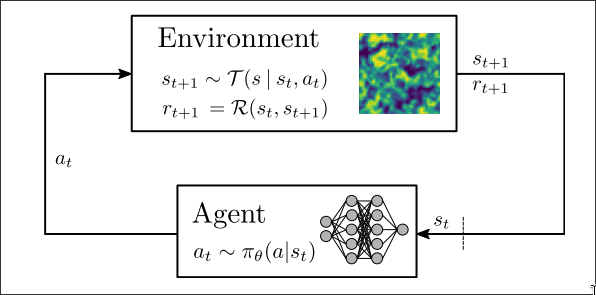
\includegraphics[width=\linewidth]{figures//Literature review/RL_LES.png}
    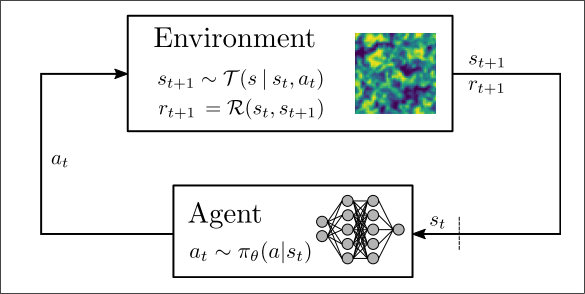
\includegraphics[width=\linewidth]{figures//Literature review/swappy-20250830-000913.png}
    \caption{The agent interacts with the LES environment to adapt the eddy viscosity dynamically based on the local flow state, adapted from \cite{Kurz2023}}
    \label{fig: RLSGS}
\end{wrapfigure}

An example of reinforcement learning being employed for developing a data-driven SGS model is the work by \textcite{Kurz2023}. This method addresses the inconsistency of supervised learning for implicitly filtered LES, where the exact form of the implicit filter is typically unknown, making it impossible to compute corresponding closure terms a priori. By formulating turbulence modelling as an RL task, the agent, based on a CNN-based policy, interacts directly with the dynamical LES environment to dynamically adapt the eddy viscosity in space and time, based solely on the local flow state. Starting from an initial flow state, the agent will keep interacting with the environment until a desirable state is reached, an overview of this process is shown in \autoref{fig: RLSGS}. The research demonstrates that the trained RL-based models achieve long-term stable simulations and significantly outperform established analytical models in accuracy, while also exhibiting strong generalizability to different resolutions and higher Reynolds numbers not seen during training.

The examples highlighted are just a few of many ML-SGS models proposed; the work by \textcite{Vinuesa2022} offers a more detailed overview of alternative proposals for the same closure problem. However, similar to the RANS closure problem, these ML-SGS still suffer from poor generalizability. This is mainly due to the limited DNS data, which is often only available at low Reynolds numbers \cite{sanderse2024}. 

\subsection{Data-Driven Reduced Order Models}
\label{subsect: data driven ROMS}
 Data-driven reduced-order models have been utilised to accelerate CFD simulations by approximating high-fidelity systems in a lower-dimensional form that retains most of the relevant flow phenomena. Data-driven ROMs extract dominant patterns from simulation or experimental snapshots without requiring explicit knowledge of the appropriate governing equations. Unlike physics-based ROMs, which typically use linear projections (such as POD) to solve the NSE on a basis with a reduced number of DOFs, data-driven ROMs rely on snapshots of the full-dimensional state vector to produce projection operations through a training process. This utilises the previously explained capabilities of neural networks to approximate a nonlinear function. These methods can achieve significant speedups after being successfully trained on supplied CFD snapshot data, or they can be used in a transfer learning fashion to accelerate CFD simulations, as will be explained in further detail. 

\begin{figure}[h]
    \centering
    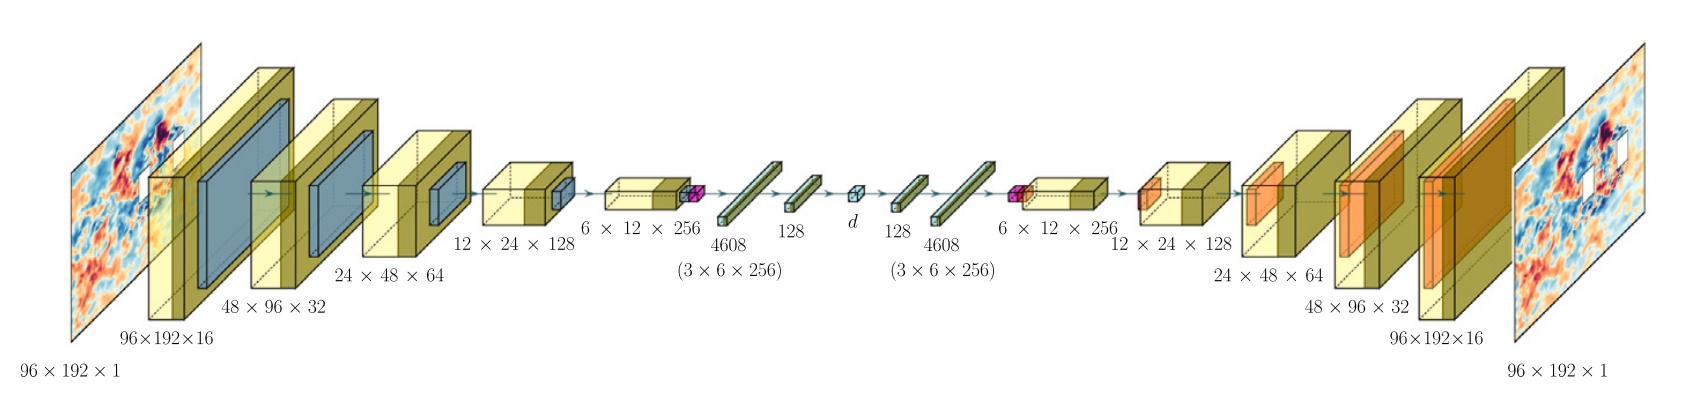
\includegraphics[width=1\linewidth]{figures//Literature review/CNN-Autoencode.png}
    \caption{Schematic view of a CNN autoencoder extracting non-linear modes from a CFD snapshot, source \cite{Eivazi2022}}
    \label{fig: CNN encoder}
\end{figure}

Data-driven ROMs employ the same working principles as autoencoders, specifically the use of the encoder and decoder network architectures. The encoder compresses the high-dimensional snapshots into a lower-dimensional latent space, and the decoder reconstructs this latent space back to the exact dimensions as the input snapshots, while minimising reconstruction error. The usage of non-linear activation functions within the autoencoder allows the network to capture the complex non-linear behaviour of turbulent structures. This offers a key advantage over methods like POD, which are limited to linear representations \cite{Pant2021}. For processing spatial data of fluid flows, autoencoders often integrate CNNs into their architecture due to their good results with grid-structured data. \autoref{fig: CNN encoder} shows an overview of how an autoencoder reduces and reconstructs a single CFD snapshot to and from a latent space. 

What differs data-driven ROMs from autoencoders is the requirement that the latent space must also capture and predict the temporal dynamics of the system. This means that, in addition to learning a compact representation of the input data, the latent variables must be predicted in a way that accurately reproduces the future state of the simulation \cite{Vinuesa2022}. This can be achieved by either selecting the dimensions of the latent space in a way that allows for a correct prediction of the future flow field, or by utilising regression architectures that are better suited for time series prediction, such as RNNs, LSTMs, or neural ODEs. 

\begin{figure}[h]
    \centering
    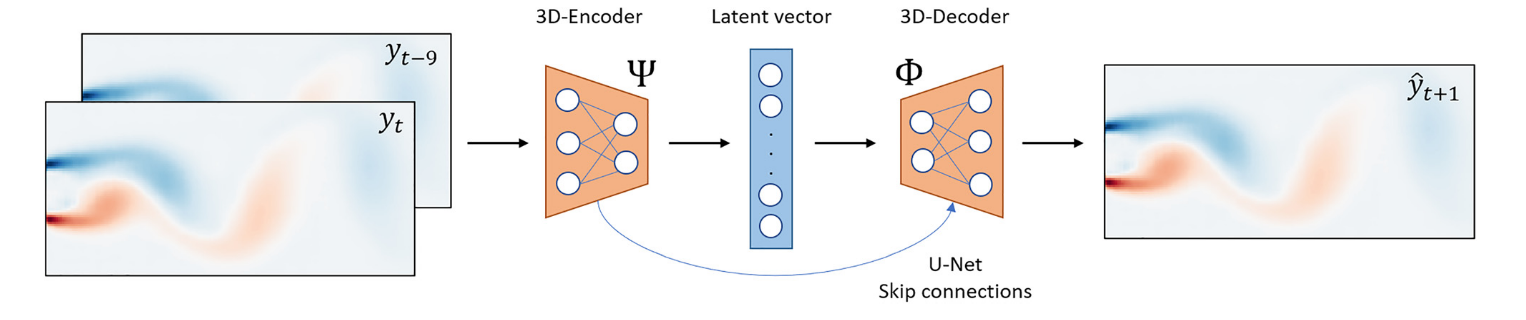
\includegraphics[width=1\linewidth]{figures//Literature review/DL-ROM.png}
    \caption{Example architecture of deep convolutional ROM, source \cite{Pant2021}}
    \label{fig: DL-ROM}
\end{figure}

Some notable examples of deep learning-based ROMs include the work of \textcite{Pant2021}, where the authors leveraged 3D Autoencoder and 3D U-Net-based architectures to create non-linear projections from reduced-order states to fluid flow snapshots, as depicted in \autoref{fig: DL-ROM}. The authors employ a looped prediction strategy, where the last 10 snapshots of a simulation are used to train the network to predict the following timestep $\hat{y}_{t+1}$. This prediction is then appended to the last nine snapshots and used as input to predict $\hat{y}_{t+2}$. This process is repeated recursively for 20 timesteps. This looping strategy allowed a reduction in simulation speed of 2 orders of magnitude \cite{Pant2021}. Similarly, CFDnet \cite{Obiols-Sales2020} accelerates RANS simulations by leveraging its CNN ROM to predict fluid properties, while still utilising the CFD solver to ensure that domain-specific convergence constraints are met. This allowed the authors to deliver highly accurate predictions while still achieving acceleration rates from 1.9 up to 7.7 times the benchmark simulations. 

\begin{wrapfigure}{r}{0.45\textwidth}
    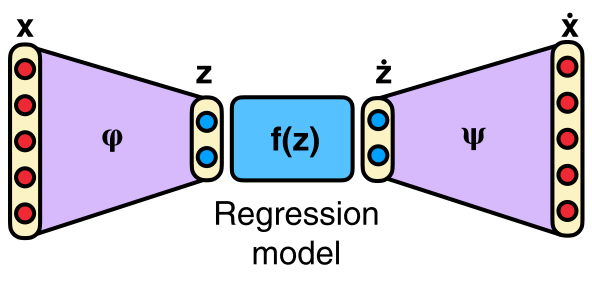
\includegraphics[width=\linewidth]{figures//Literature review/DL-regression-ROM.png}
    \caption{Example architecture of autoencoder with regression in the latent space, adapted from \cite{Vinuesa2022}}
    \label{fig: ROM regressor}
\end{wrapfigure}

As previously mentioned, the dynamics in the latent space can also be modelled by utilising a regressor in the latent space of the autoencoder, which would make the architecture of the data-driven ROM look like \autoref{fig: ROM regressor}. A notable example of such an architecture is the work by \textcite{Shankar2022}, which demonstrates how NODEs are utilised to model system dynamics in the latent space. By explicitly decoupling the reduction and latent system dynamics, the presented framework achieved very accurate reconstructions of flow dynamics over large integral timescales. Instead of using NODEs for the dynamical modelling in the latent space, LSTMs can also be used, as they present good capabilities for time series predictions, as indicated in the work by \textcite{Mohan2019}.

\subsection{Physics Informed Surrogate Models}
\label{subsect: PIsurrogates}
Physics-informed surrogate models demonstrate strong potential in accelerating computationally intensive simulations. A surrogate model is a broad term for a computationally efficient approximation of a complex system. A ROM, which was handled previously, is a specific type of surrogate that reduces the system's dimensionality by applying a projection to the high-dimensional dynamics in a lower-dimensional space. Meaning that all ROMS are essentially surrogate models, not all surrogates are ROMS. 

Where purely data-driven surrogate models, such as DeepONet \cite{Lu2021}, require a large amount of data for reliable prediction performance. In real-world scenarios, where data is either sparse or prohibitively expensive to collect, models that can generalise effectively on smaller datasets are necessary \cite{Donnelly2024}. That is why physics-informed surrogate models embed fundamental physical laws and constraints directly into their architecture or training process. This integration aims to create efficient approximations that are not only accurate but also physically consistent, even when dealing with limited training data \cite{Raissi2019}. 

The integration of physics into these models is achieved mainly through two key mechanisms: physics-informed loss functions and specialised network architecture. Physics-informed loss functions incorporate the residuals of the governing partial differential equations, such as conservation of mass \ref{eq: continuity} and momentum \ref{eq: momentum}, into the loss function during training. This way, the model can be regularised during training, showing bigger errors for predictions which violate the relevant physical laws. Essentially, an artificial bias is added to the network, which promotes data efficiency since the projections are inherently directed to adhere to physical laws. \autoref{eq: physicsloss} shows a general form of a physics-informed loss function, where $\mathcal{L}_{\text{data}}$ is a standard loss function like MSE or MAE, and $\mathcal{L}_{\text{physics}}$ can be derived from the physical system the network has to learn. In the case of a CFD simulation, this latter part can be built from the continuity and momentum equations. These two loss functions can then be combined using a weighted sum, with $\lambda_d$ and $\lambda_p$ serving as weights.

\begin{equation}\label{eq: physicsloss}
\mathcal{L} = \lambda_d \, \mathcal{L}_{\text{data}} 
+ \lambda_p \, \mathcal{L}_{\text{physics}} 
\end{equation}

A prominent example is Physics Informed Neural Networks (PINNs), first proposed by \textcite{Raissi2019}, that use deep learning to solve PDEs, exploiting the concept of automatic differentiation used in the back propagation algorithm to calculate partial derivatives \cite{Vinuesa2022}. PINNs have been utilised in various CFD scenarios, including hydrodynamic surrogate models \cite{Donnelly2024}, high-speed flow approximations \cite{Mao2020}, and more general NS cases \cite{Eivazi2021, Sun2019}, where they have demonstrated excellent results in predicting flow parameters with limited training data. However, in the context of accelerating fluid simulations, PINNs have a disadvantage in that their training speed restricts them from achieving significant speed-up results in a CFD workflow \cite{Jeon2024, Go2023}. On the other hand, PINNs have been successfully used as closure models for RANS and LES frameworks; the workings of this will be explained later in this literature review. 

Alternatively to PINNs, the Finite Volume Method Network FVMN \cite{Jeon2022} is a physics-informed surrogate model which specifically exemplifies a physics-informed surrogate model tailored for CFD, integrating principles of the finite volume method (FVM) directly into its design. Unlike previously explained methods that only include information about a single grid point, FVMN employs a tiered input system that incorporates physical quantities from a central grid point and its neighbouring grid points into the input matrix of the neural network. This allows the network to imitate the mass and heat transport among neighbouring cells, which is considered the most crucial process in the FVMN. Additionally, instead of directly predicting the future state, FVMN employs a derivative output system, which means it predicts the change or derivative of physical quantities over a given time step. 

\begin{figure}[h]
    \centering
    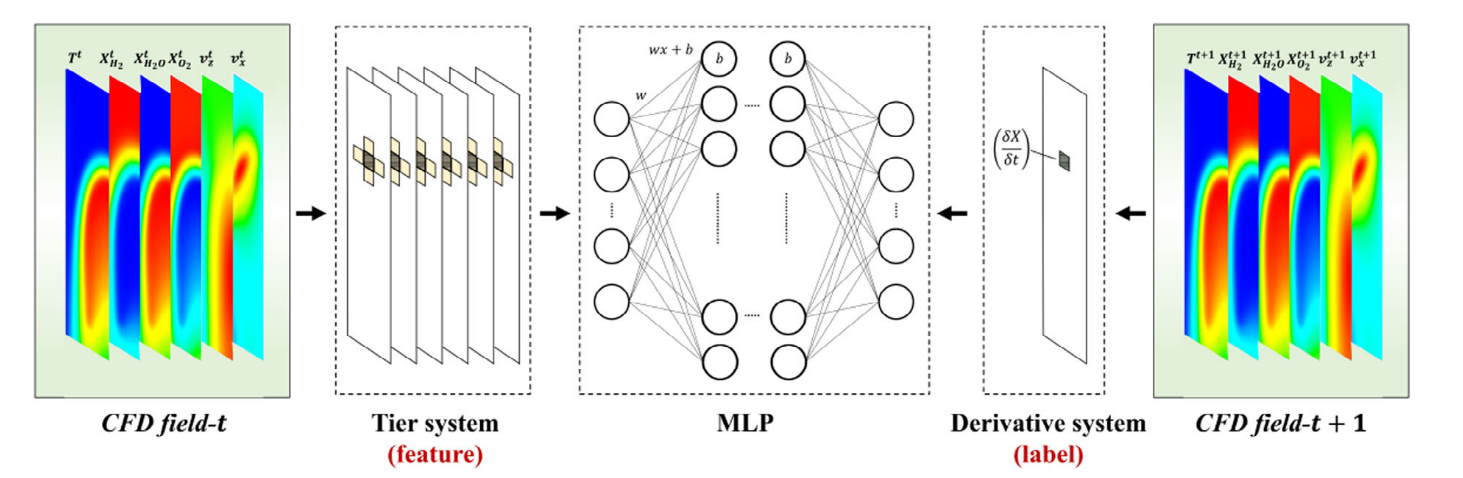
\includegraphics[width=1\linewidth]{figures//Literature review/FVMN.png}
    \caption{Overview of the FVMN architecture, showing the tier-derivative input/output system built around a conventional FFN (or MLP), adapted from \cite{Jeon2022}}
    \label{fig: FVMN}
\end{figure}

In the original work \textcite{Jeon2022}, significant improvements in accuracy were showcased compared to general models without the tier/derivative system implemented, where the authors managed to achieve a relative error with respect to CFD data of not more than 0.05\%, compared to 1.12\% for the conventional model.

In the context of accelerating CFD simulations, the FVMN also showed promising results. Due to the system's linearly increasing gradient error when used for longer transient predictions, the authors proposed an ML-CFD cross-coupling framework. The Residual-based Physics Informed Transfer learning strategy (RePIT) \cite{Jeon2024} is a hybrid framework where both a CFD solver and the FVMN alternately predict time series of fluid flows. RePIT continuously monitors the residuals of the governing equations, NSE \ref{eq: navier-stokes}, which are part of the physics-informed loss function employed by the FVMN in the case of fluid flows. \autoref{fig: RePIT} shows a schematic overview of the transfer learning framework, it shows that when the residuals of the loss function ($\varepsilon$) exceed a predefined tolerance ($\varepsilon_{th}$), the CFD solver will use the latest prediction and continue solving the governing equations to reduce the residuals back to a desired value. Afterwards, these newly computed CFD snapshots are used to update the network parameters, allowing for new predictions to be made. 

\begin{figure}[H]
    \centering
    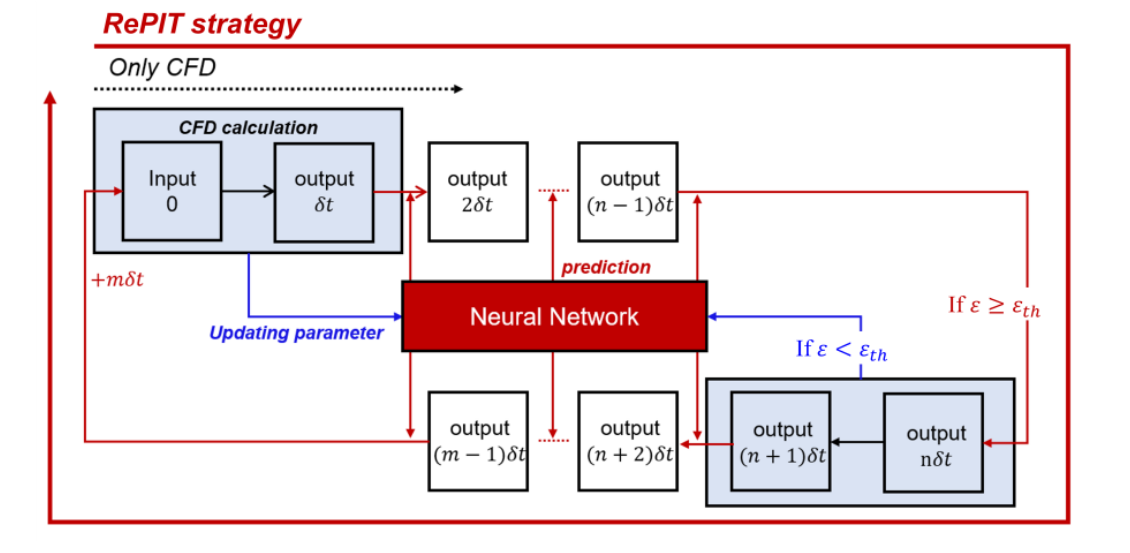
\includegraphics[width=1\linewidth]{figures//Literature review/RePIT.png}
    \caption{Schematic overview of the RePIT strategy showing the transfer learning process, adapted from \cite{Jeon2024}}
    \label{fig: RePIT}
\end{figure}

This framework leads to significant computational speed-ups without compromising accuracy. The authors implemented this method in a natural convection CFD case, achieving a 1.9 times acceleration, including network parameter updates. This demonstrates the strong capabilities of the FVMN, as its tier-based input system requires a minimal amount of training data. RePIT shows strong potential as it is universally adaptable to various flow cases and boundary conditions. 

While RePIT and FVMNs approximate spatial derivatives using mesh-based network structures, they can achieve smoother predictions by enabling the functionality of a continuous integrator, such as NODEs. Embedding NODEs into the RePIT framework would merge its residual-based transfer learning with NODEs’ ability to handle adaptive time integration and irregular sampling. This combination has the potential to enhance stability, improve generalisation across flow regimes, and further reduce the computational cost of turbulent CFD simulations

\pagebreak

\subsection{Challenges and Future Directions}

Machine learning has presented interesting solution paradigms for accelerating CFD simulations across various fronts. The most promising direction is the development of hybrid ML-CFD methods. Where traditional CFD solvers and ML models alternate between calculating/predicting time series data, methods like RePIT \cite{Jeon2024} and CFDNet \cite{Obiols-Sales2020} demonstrate that, when training data and loss functions are controlled, error accumulation can be mitigated, yielding significant speedups. Their online operation also enables the transferability of hybrid methods to a range of flow cases, making them more applicable to real-world CFD workflows. 

The ML-enhanced CFD field is also showing promising advances through more sophisticated architectures and loss functions. Frameworks such as PINNs \cite{Raissi2019} and PNODEs \cite{Sholokhov2023} can enforce physical constraints, such as incompressibility, and learn from observational data to provide accurate predictions of complex flow fields. It can therefore be argued that the embedding of physical laws into neural network architecture is an essential feature for future acceleration frameworks.

Despite these advancements, key challenges and opportunities remain in the field. One of these is the interpretability of the ML models. Due to their often complex nature, ML models tend to be a black box model. This opaqueness hinders their performance as effectively as physics-based models, making it difficult to understand why a model made a specific prediction \cite{Vinuesa2022, Girimaji2024}. This is a critical issue for generalisation, as models trained solely on data may struggle with unseen geometries and flow conditions, or when extrapolating beyond the training data's probability distribution. While advancements in hardware architecture \cite{ansys2023multiGPU, Chen2009} and automatic data generation continue to aid in providing the high-quality datasets needed for these models, the ultimate goal is to enable ML to not only accelerate simulations but also advance discoveries of new physical mechanisms and revisit empirical laws in fluid mechanics through more transparent and quantifiable models. 

While efforts continue for automatic data generation and automated experimentation pipelines to provide the large, high-quality datasets needed, the ultimate goal is to enable ML to not only accelerate simulations but also to assist in discovering new physical mechanisms and revisiting existing empirical laws in fluid mechanics, by yielding more transparent and certifiable models \cite{Brunton2020, Vinuesa2022}.

Despite the numerous advancements made in applying machine learning to CFD, the current literature still reveals several limitations. Many studies have employed NODEs only within reduced-order models \cite{Rojas2021, Shankar2022}, rather than integrating them directly into the CFD solver to accelerate the core time-integration step. Notably, their ability to serve as continuous time integrators has not been fully leveraged in scale-resolved simulations. That is why this work proposes applying a similar method to the RePIT framework by replacing its FVMN with NODEs. The RePIT framework showed that long-term stable acceleration can be achieved by alternating between CFD and machine learning predictions, guided by residual monitoring of the governing equations. The implementation of NODEs into the RePIT strategy can thus leverage RePIT’s residual-based transfer learning, complemented by NODEs’ continuous-time formulation. This strategy aims to directly address the bottleneck of time integration in CFD solvers, while ensuring that physical consistency is maintained through the use of residual monitoring. By pursuing this integration, the framework seeks to provide a concrete answer to the research questions introduced earlier: whether NODEs can deliver solver-level acceleration without compromising accuracy, and how residual monitoring can make such integration feasible.
